\chapter{Результаты}

В этой главе приведены результаты спектрального анализа промежуточных представлений моделей ResNet, ViT и Swin. В главе отдельно рассматриваются два типа материалов: радиальные спектральные кривые и сводные численные метрики, рассчитанные по этим кривым. Такой порядок позволяет сначала проанализировать форму спектра визуально, а затем проверить те же наблюдения через центроид, долю низкочастотной энергии и скорость спектрального сжатия.

Для визуализации берётся средняя мощность в кольце, затем каждая кривая нормируется на свой максимум для сравнимости формы. Поэтому по ним сравнивается не абсолютная величина энергии, а форма радиального распределения. Полупрозрачные области вокруг линий показывают разброс значений по изображениям выборки. Для численных таблиц ниже используются уже не радиальные средние значения, а суммарная энергия по кольцам; это важно, потому что только так доля низкочастотной энергии действительно учитывает число точек в каждом радиальном диапазоне.

\section{Спектральные кривые}

\subsection{Динамика внутри ResNet}

На Рис. \ref{fig:ResNet18} показано, как меняется радиальный спектр мощности при переходе от \texttt{layer1} к \texttt{layer4} в ResNet18. Здесь хорошо видна характерная для свёрточной сети картина: ранний уровень даёт более широкий спектр, а поздние уровни постепенно стягивают энергию к области малых частотных радиусов. У \texttt{layer1} хвост кривой длиннее. Это значит, что в представлении ещё остаётся заметная доля средне- и высокочастотных компонент, которые могут соответствовать границам, текстурам и мелким локальным изменениям.

Дальше спектр становится уже. На \texttt{layer2} и \texttt{layer3} вклад более высоких частот уменьшается, а на \texttt{layer4} кривая занимает уже ограниченный участок частотной оси. По сути, слой всё меньше похож на представление с большим количеством локальных деталей и всё больше — на сглаженное описание крупных структур. Но здесь нужно быть аккуратным: в ResNet при переходе между стадиями уменьшается пространственное разрешение. Значит, часть сужения спектра может быть обычным следствием понижения разрешения, а не только свойством обученных признаков.

ResNet18 на этом графике даёт удобный базовый пример низкочастотной динамики в свёрточной сети. Ранние карты признаков сохраняют широкий частотный диапазон, поздние — переходят к более узкому описанию. Доказательность этого вывода проверяется ниже через контрольный эксперимент: реальный глубокий слой сравнивается с ранним слоем, искусственно приведённым к тому же пространственному размеру.

\begin{figure}[h]
    \centering
    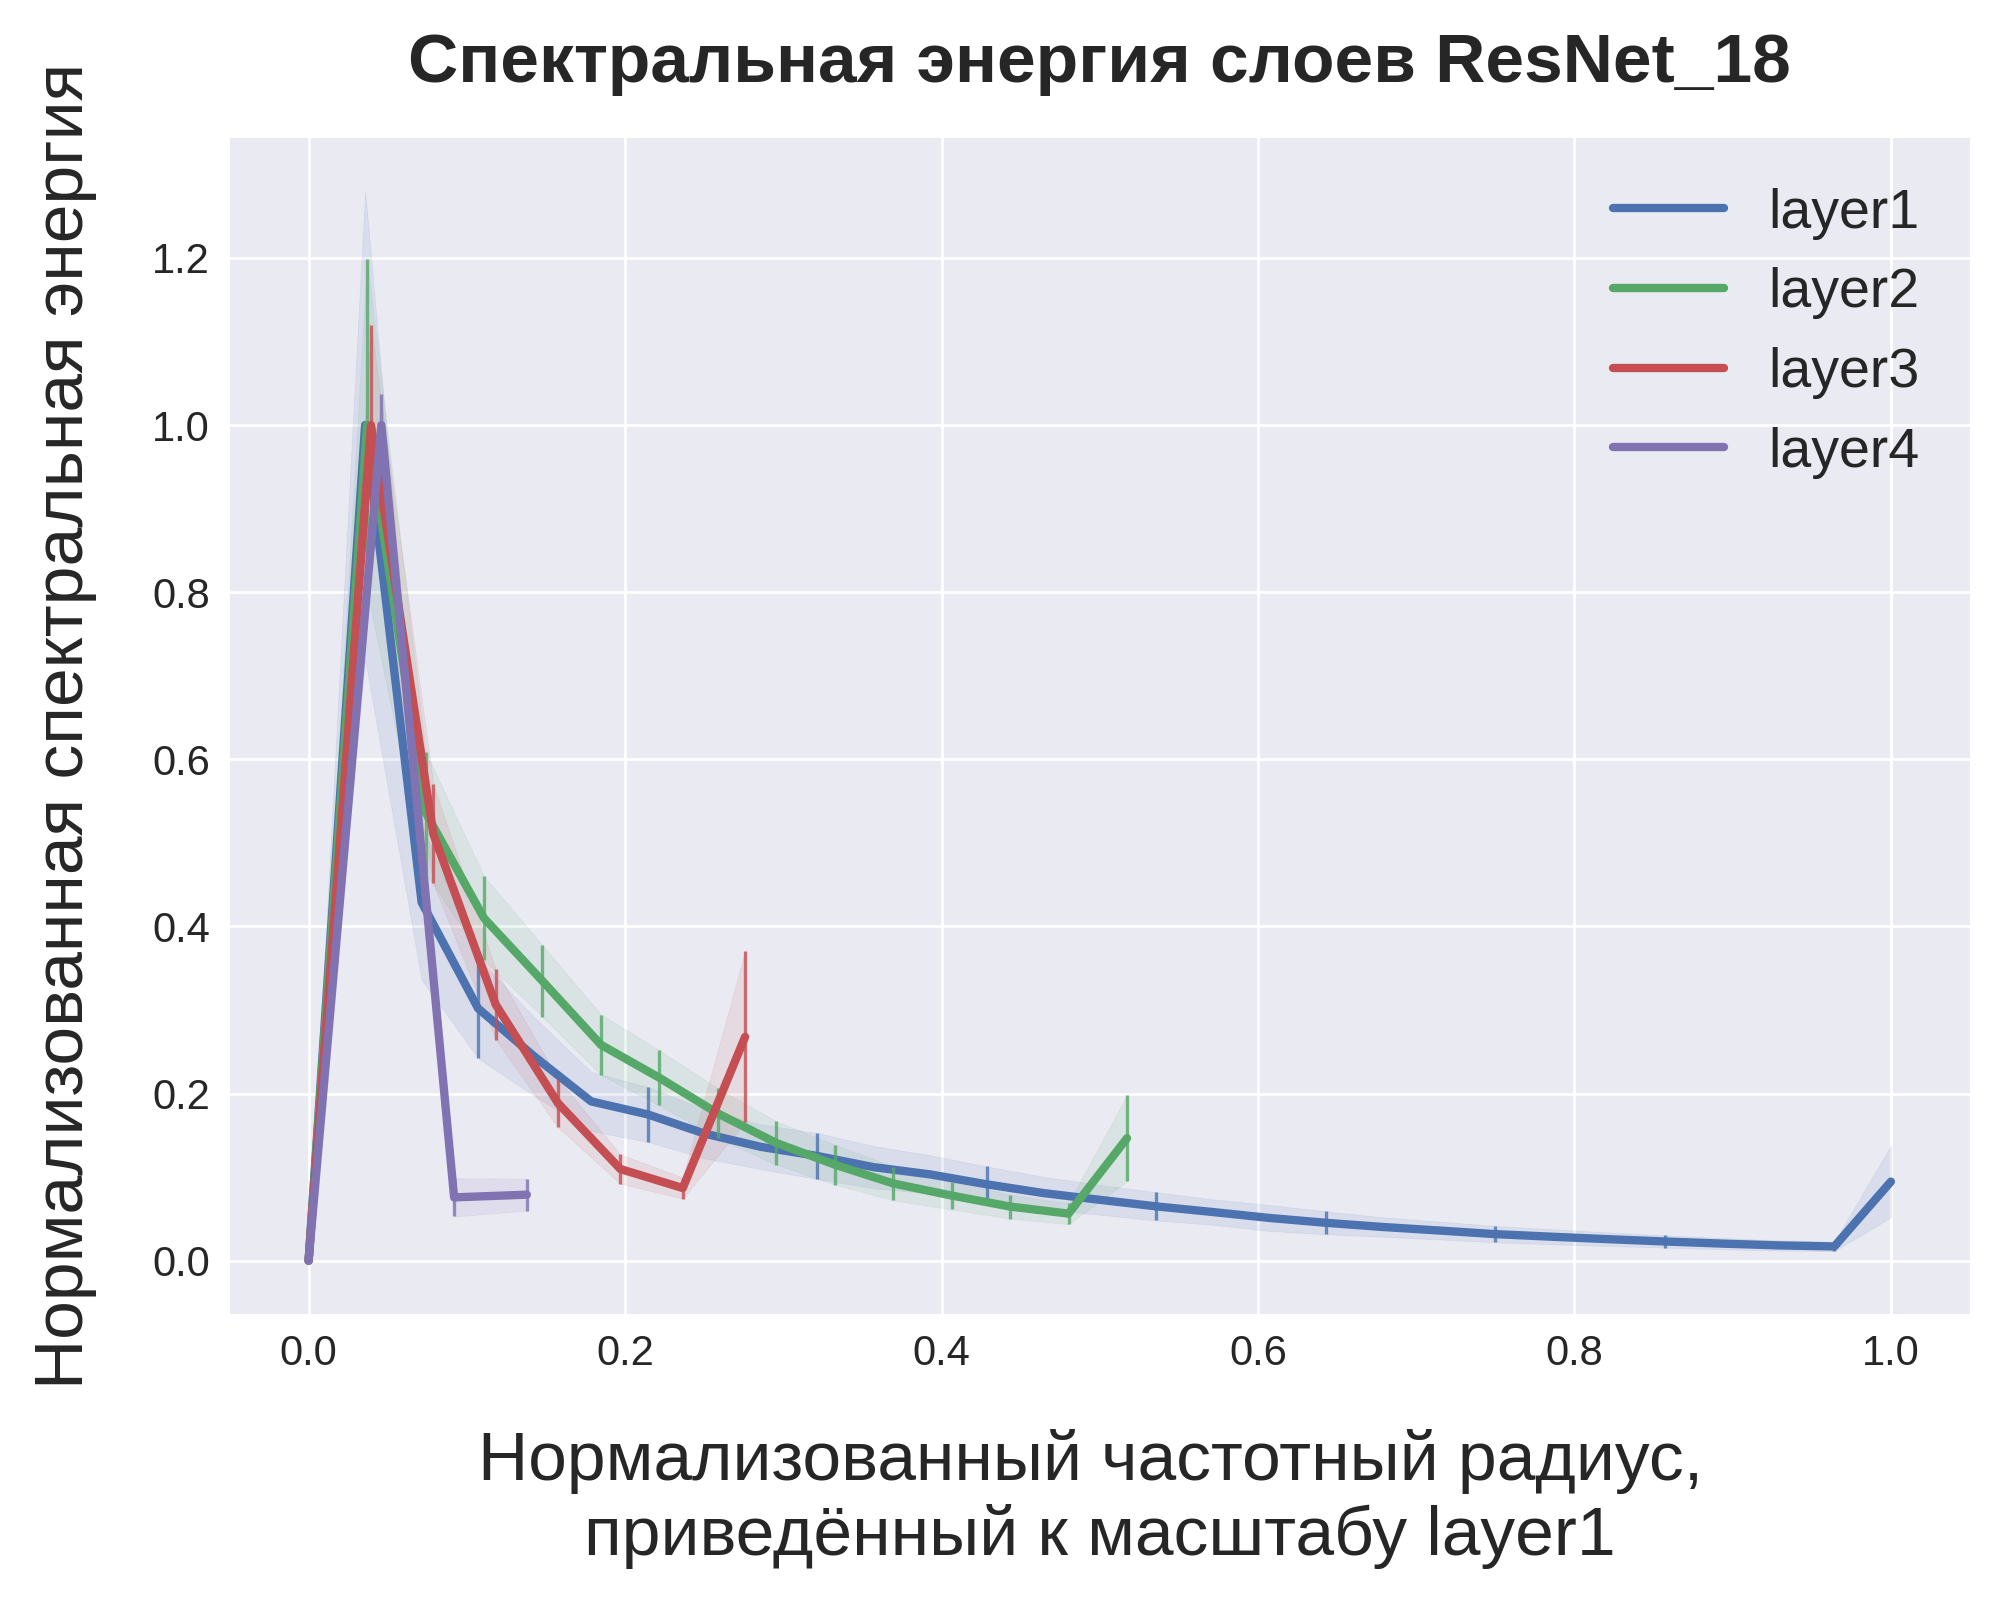
\includegraphics[width=0.8\textwidth]{figures/ResNet_18_spectra_layers.png}
    \caption{Изменение спектрального профиля по слоям ResNet18.}
    \label{fig:ResNet18}
\end{figure}

На Рис. \ref{fig:resnet_downsampling_control_layer4} приведён контрольный эксперимент для ResNet18. Сравниваются реальный \texttt{layer4} и представление \texttt{layer1}, искусственно уменьшенное до размера \texttt{layer4}. Если бы наблюдаемое сужение спектра объяснялось только уменьшением разрешения, эти две кривые должны были бы быть близки.

\begin{figure}[h]
    \centering
    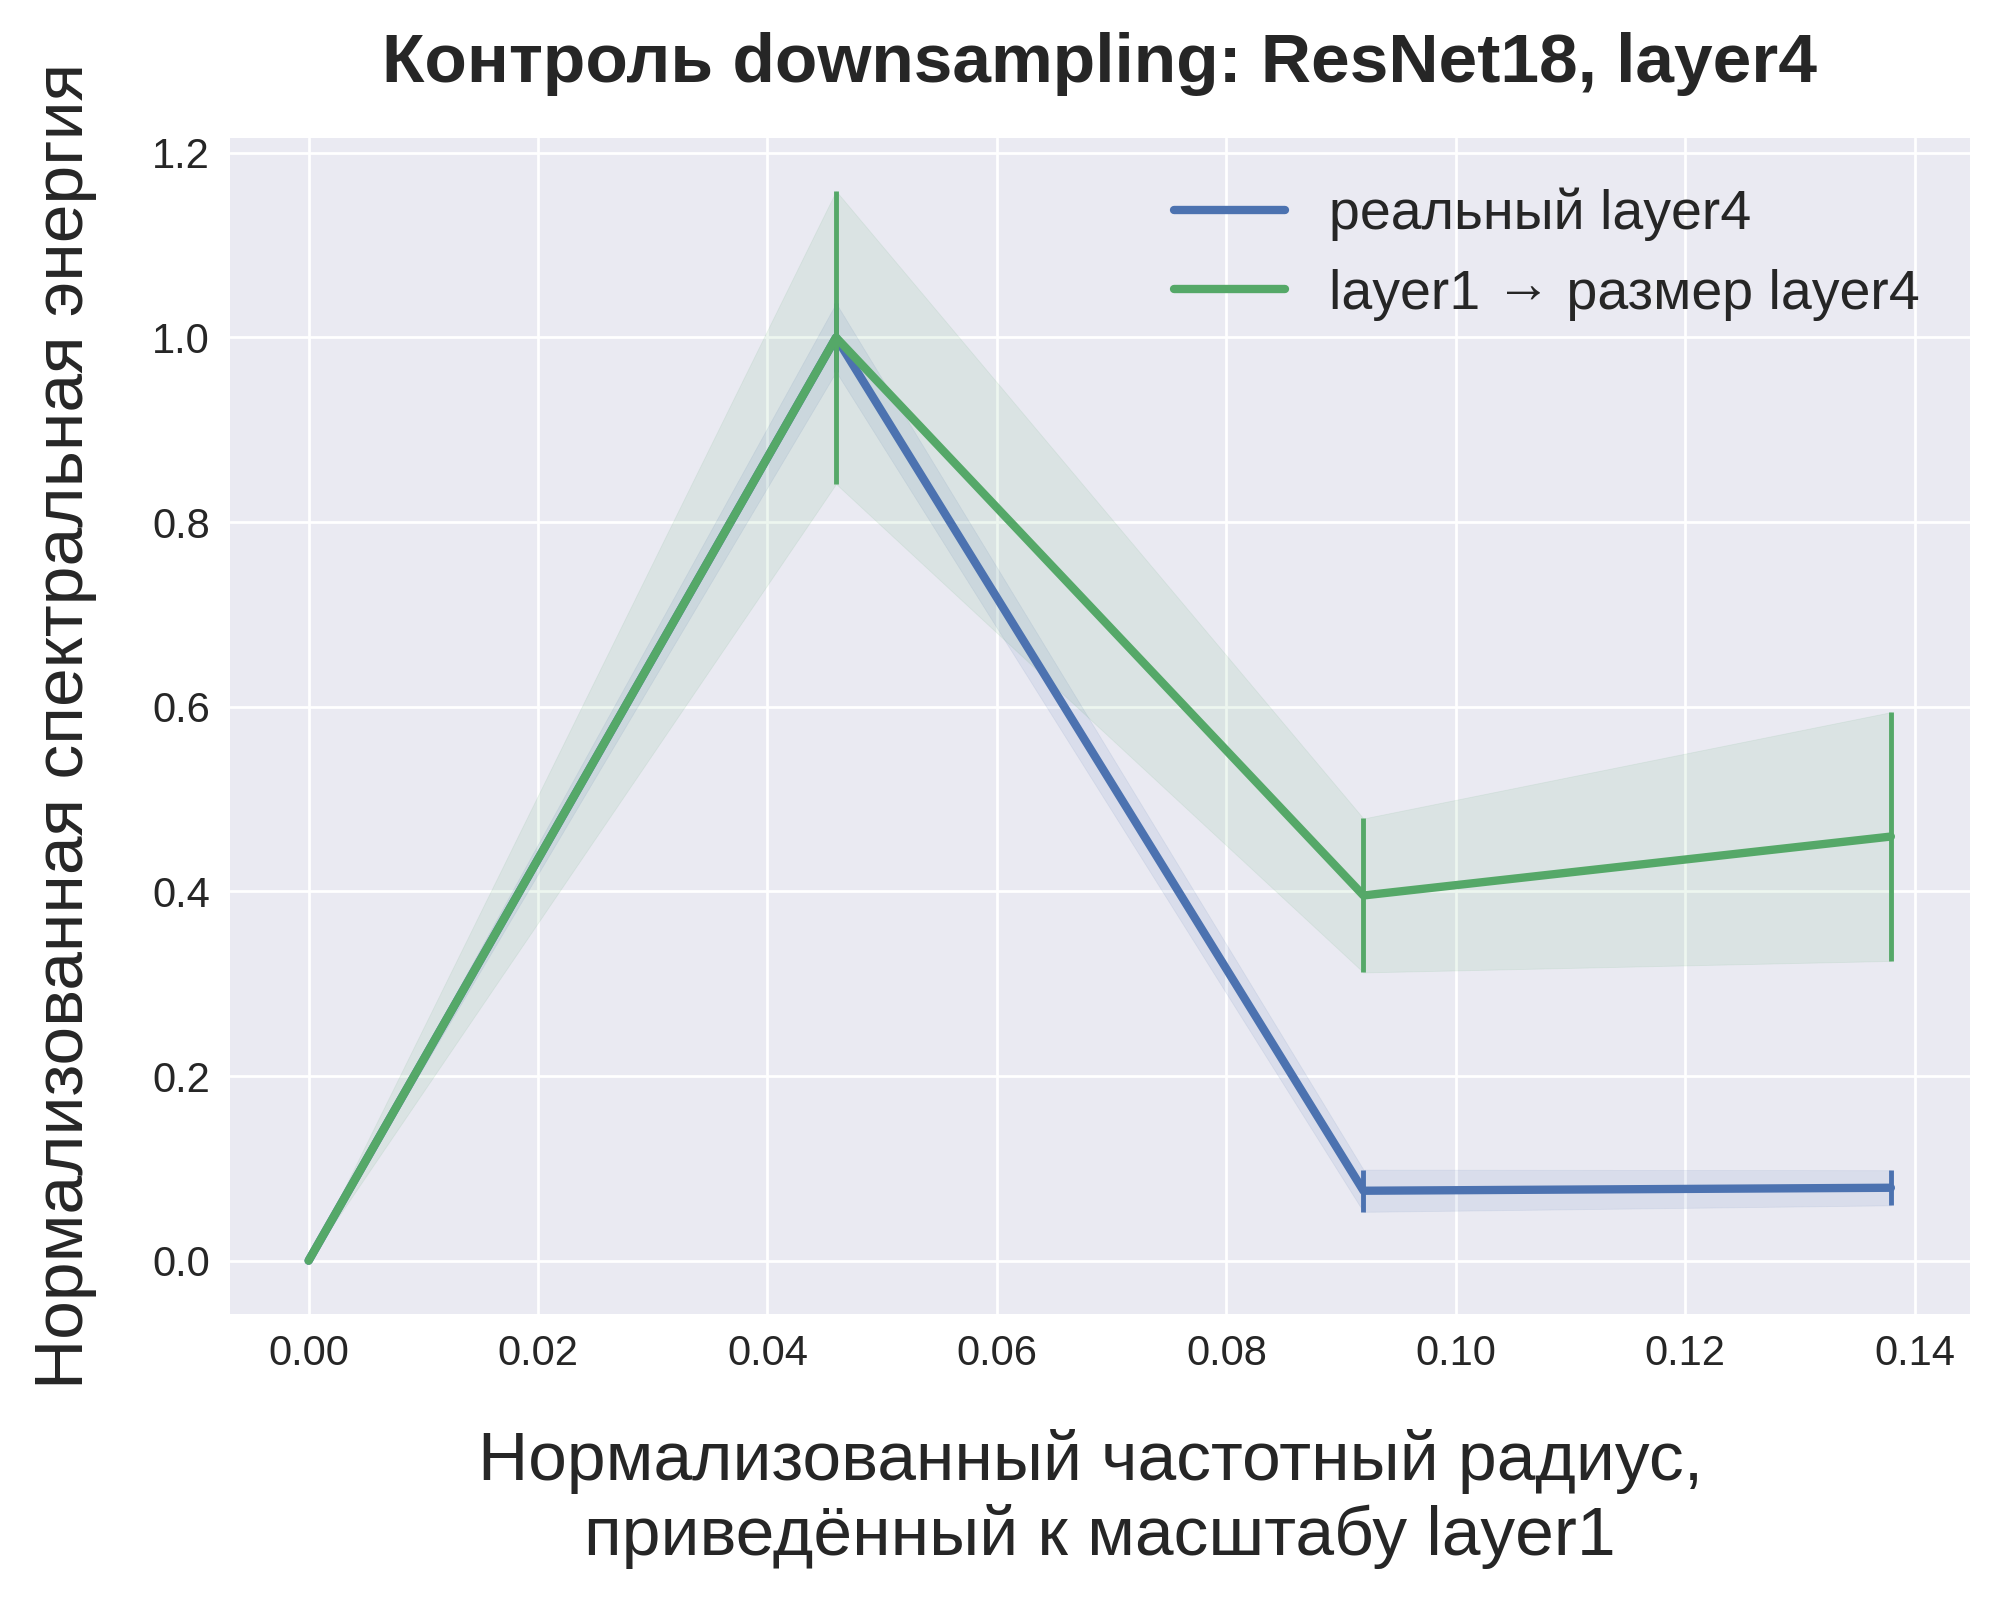
\includegraphics[width=0.8\textwidth]{figures/resnet18_downsampling_control_layer4.png}
    \caption{Контроль влияния понижения разрешения для ResNet18: сравнение реального \texttt{layer4} и \texttt{layer1}, приведённого к размеру \texttt{layer4}.}
    \label{fig:resnet_downsampling_control_layer4}
\end{figure}

На графике видно другое. Искусственно уменьшенный \texttt{layer1} сохраняет более высокий хвост в правой части частотного диапазона. Реальный \texttt{layer4} после низкочастотного пика падает заметно резче и почти не сохраняет энергии в более высоких радиусах. Таким образом, это главный контроль для ResNet: одно только уменьшение пространственного размера не воспроизводит форму глубокого слоя. Значит, в ResNet есть дополнительное изменение спектрального профиля сверх простого понижения разрешения.

На Рис. \ref{fig:resnet50_layer3_within_stage_control} показан второй контроль — сравнение блоков внутри \texttt{layer3} модели ResNet50. Эти блоки имеют одинаковое пространственное разрешение, поэтому различия между ними уже нельзя объяснить переходом к меньшей карте признаков.

\begin{figure}[h]
    \centering
    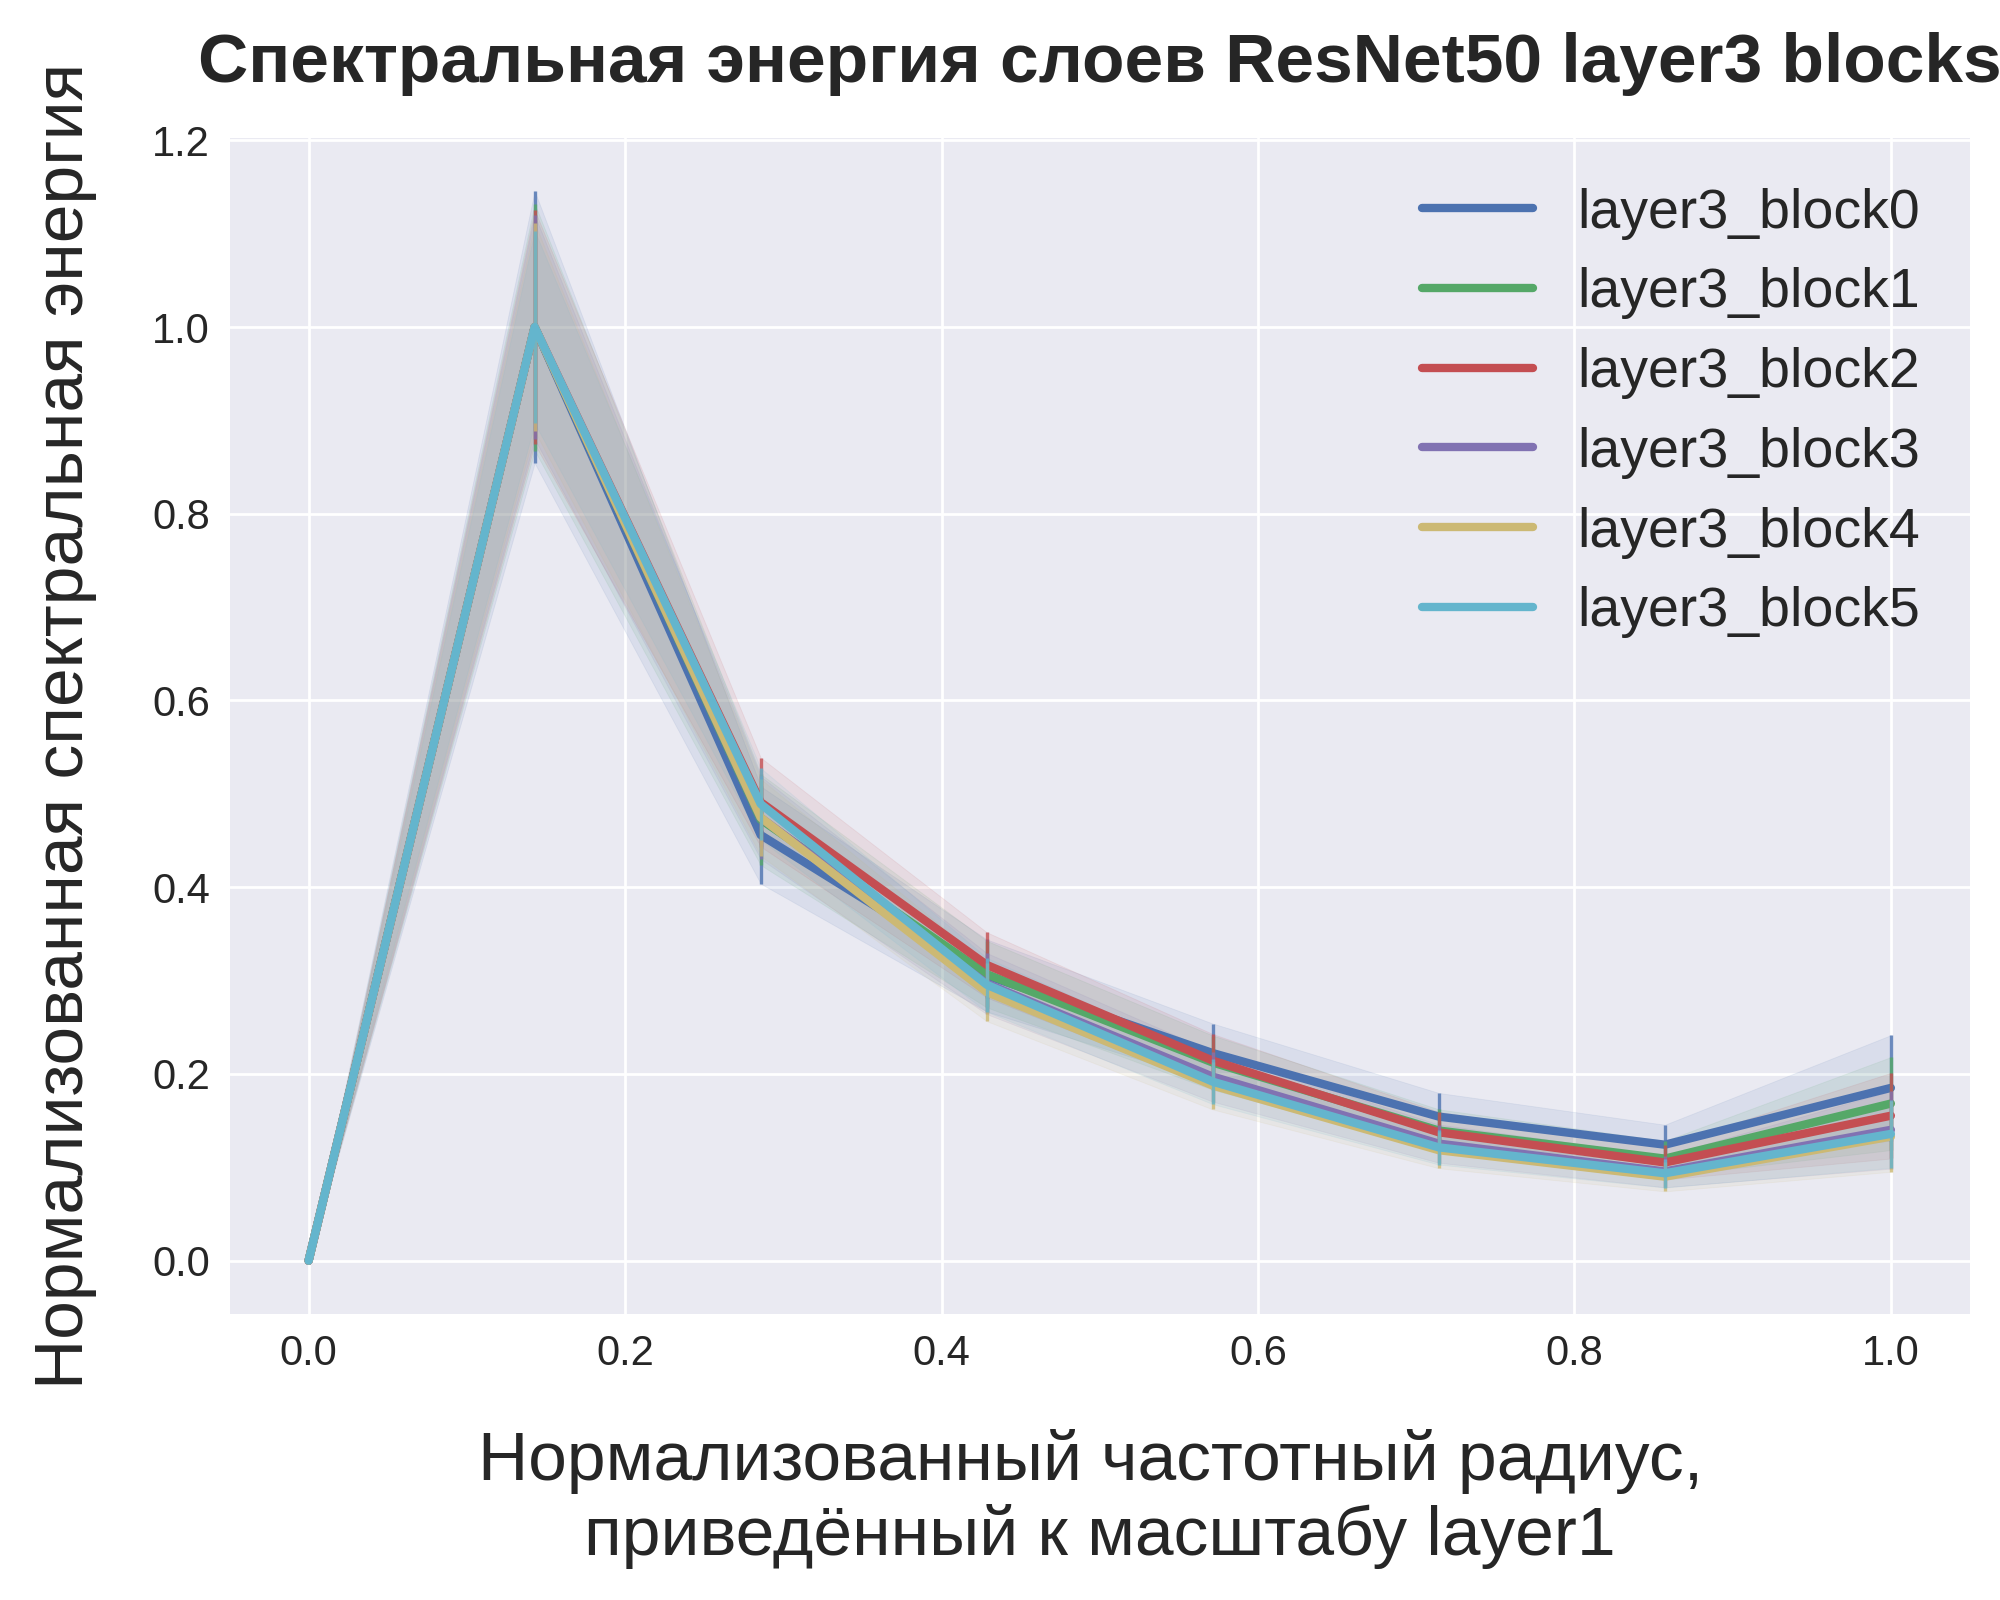
\includegraphics[width=0.8\textwidth]{figures/resnet50_layer3_within_stage_control.png}
    \caption{Внутристадийный контроль для ResNet50: спектральные профили блоков внутри \texttt{layer3} при фиксированном пространственном разрешении.}
    \label{fig:resnet50_layer3_within_stage_control}
\end{figure}

Кривые внутри стадии очень близки. Небольшие отличия есть, но они намного слабее, чем различия между \texttt{layer1}, \texttt{layer2}, \texttt{layer3} и \texttt{layer4}. Это уточняет вывод: наиболее резкая часть спектральной динамики ResNet связана именно с межстадийными переходами и накопленным изменением признаков. Внутри одной стадии при фиксированном разрешении спектр меняется гораздо спокойнее.

\subsection{Динамика внутри ViT}

На Рис. \ref{fig:vit_large_spectra_layers} приведены спектральные кривые выбранных блоков ViT-Large. По сравнению с ResNet поведение здесь другое. Не видно простого движения, при котором каждый следующий блок всё сильнее сжимает спектр к низким частотам. Напротив, поздние блоки ViT-Large сохраняют более заметный вклад в области средних частот. Особенно хорошо это видно по \texttt{block\_17} и \texttt{block\_23}: спад у них более пологий, а хвост остаётся выше, чем у ранних блоков.

\begin{figure}[h]
    \centering
    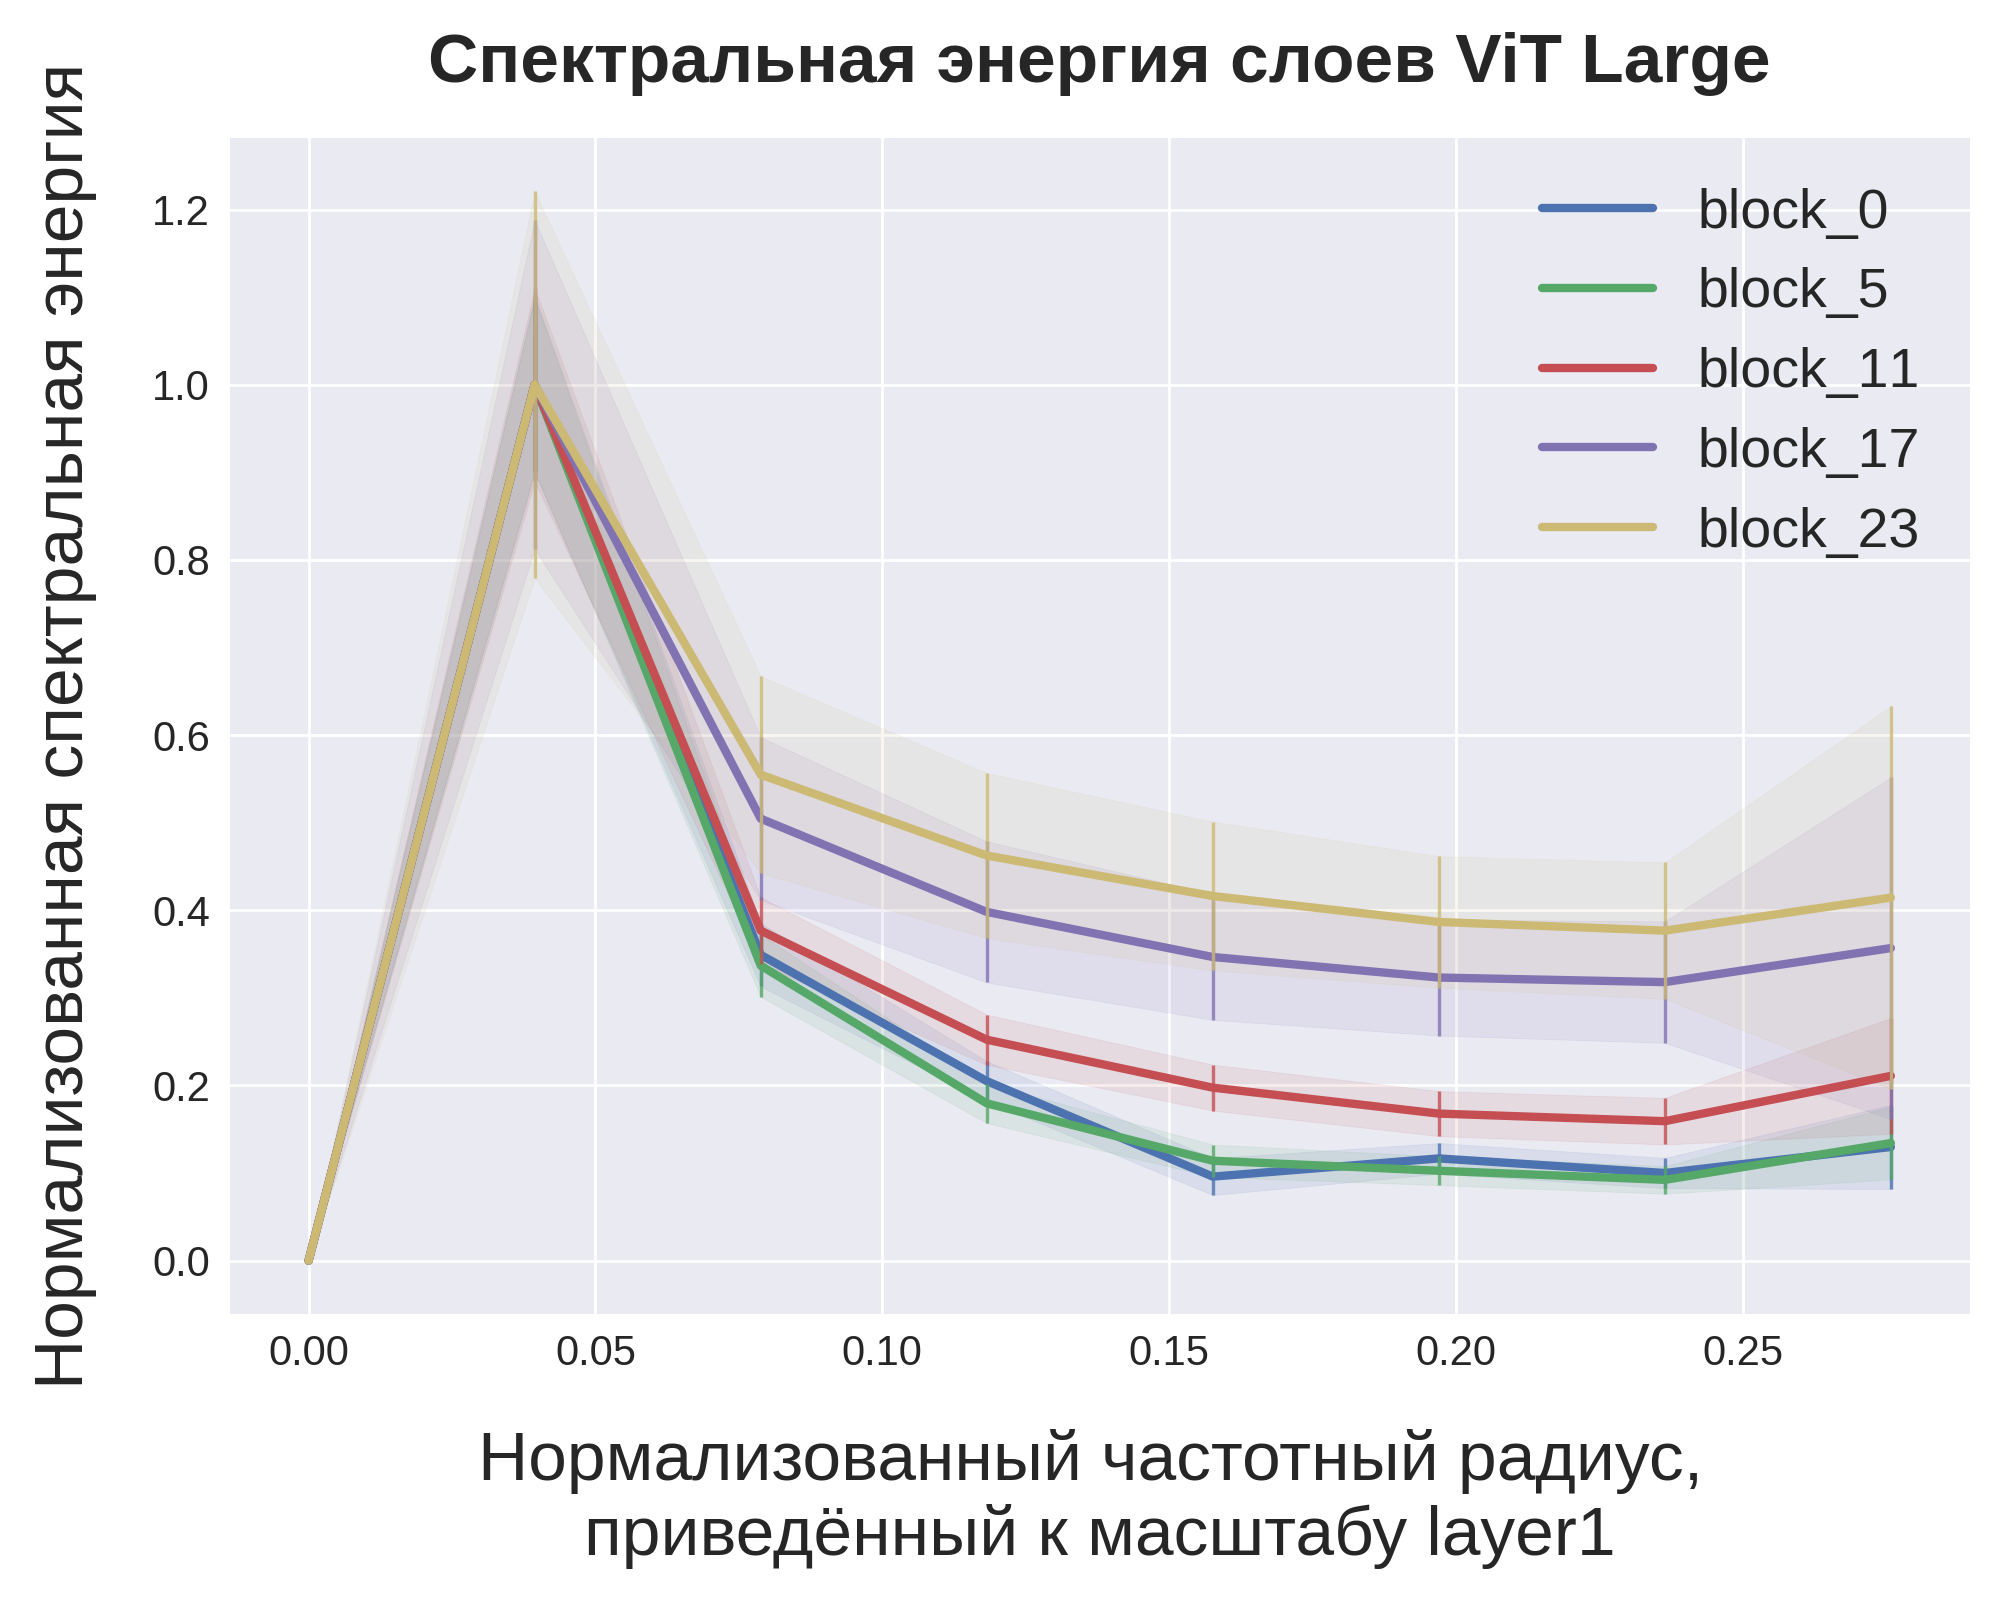
\includegraphics[width=0.8\textwidth]{figures/vit_large_spectra_layers.png}
    \caption{Изменение спектрального профиля по блокам ViT-Large.}
    \label{fig:vit_large_spectra_layers}
\end{figure}

Это наблюдение методически удобно: в стандартном ViT размер патчевой решётки не уменьшается от блока к блоку. Поэтому изменения между блоками нельзя списать на межстадийное понижение разрешения, как это приходится делать для ResNet и Swin. Здесь мы видим именно изменение токенных представлений на фиксированной пространственной решётке.

При этом более широкий хвост не стоит читать как прямое доказательство лучшего сохранения полезной семантики. График говорит о другом: в выбранном протоколе ViT-Large не демонстрирует устойчивого низкочастотного сжатия. Что именно несёт энергия в среднечастотной области — полезные детали, особенности токенного кодирования или побочные вариации, — требует отдельного анализа. В данной работе фиксируется сам факт: динамика ViT не похожа на последовательное подавление более высоких частот.

\subsection{Динамика внутри Swin}

На Рис. \ref{fig:swin_large_spectra_layers} показана динамика выбранных блоков Swin-Large. Начальный блок \texttt{stage0\_block0} имеет резкий низкочастотный пик и быстро убывающий хвост. Далее картина становится менее прямой: на блоках \texttt{stage2} часть кривых расширяется и сохраняет заметную энергию в среднечастотной зоне. Финальный \texttt{stage3\_block1} снова расположен в более узком диапазоне.

Swin, таким образом, не повторяет ResNet один к одному. У него есть иерархическая структура и операция объединения патчей, но средние стадии ведут себя сложнее. Возможное объяснение связано с оконной обработкой и изменением локальных взаимодействий между токенами. Однако это именно интерпретация, а не отдельный причинный эксперимент. Поэтому дальше я проверяю, насколько финальное сужение Swin можно объяснить одним только уменьшением разрешения.

\begin{figure}[h]
    \centering
    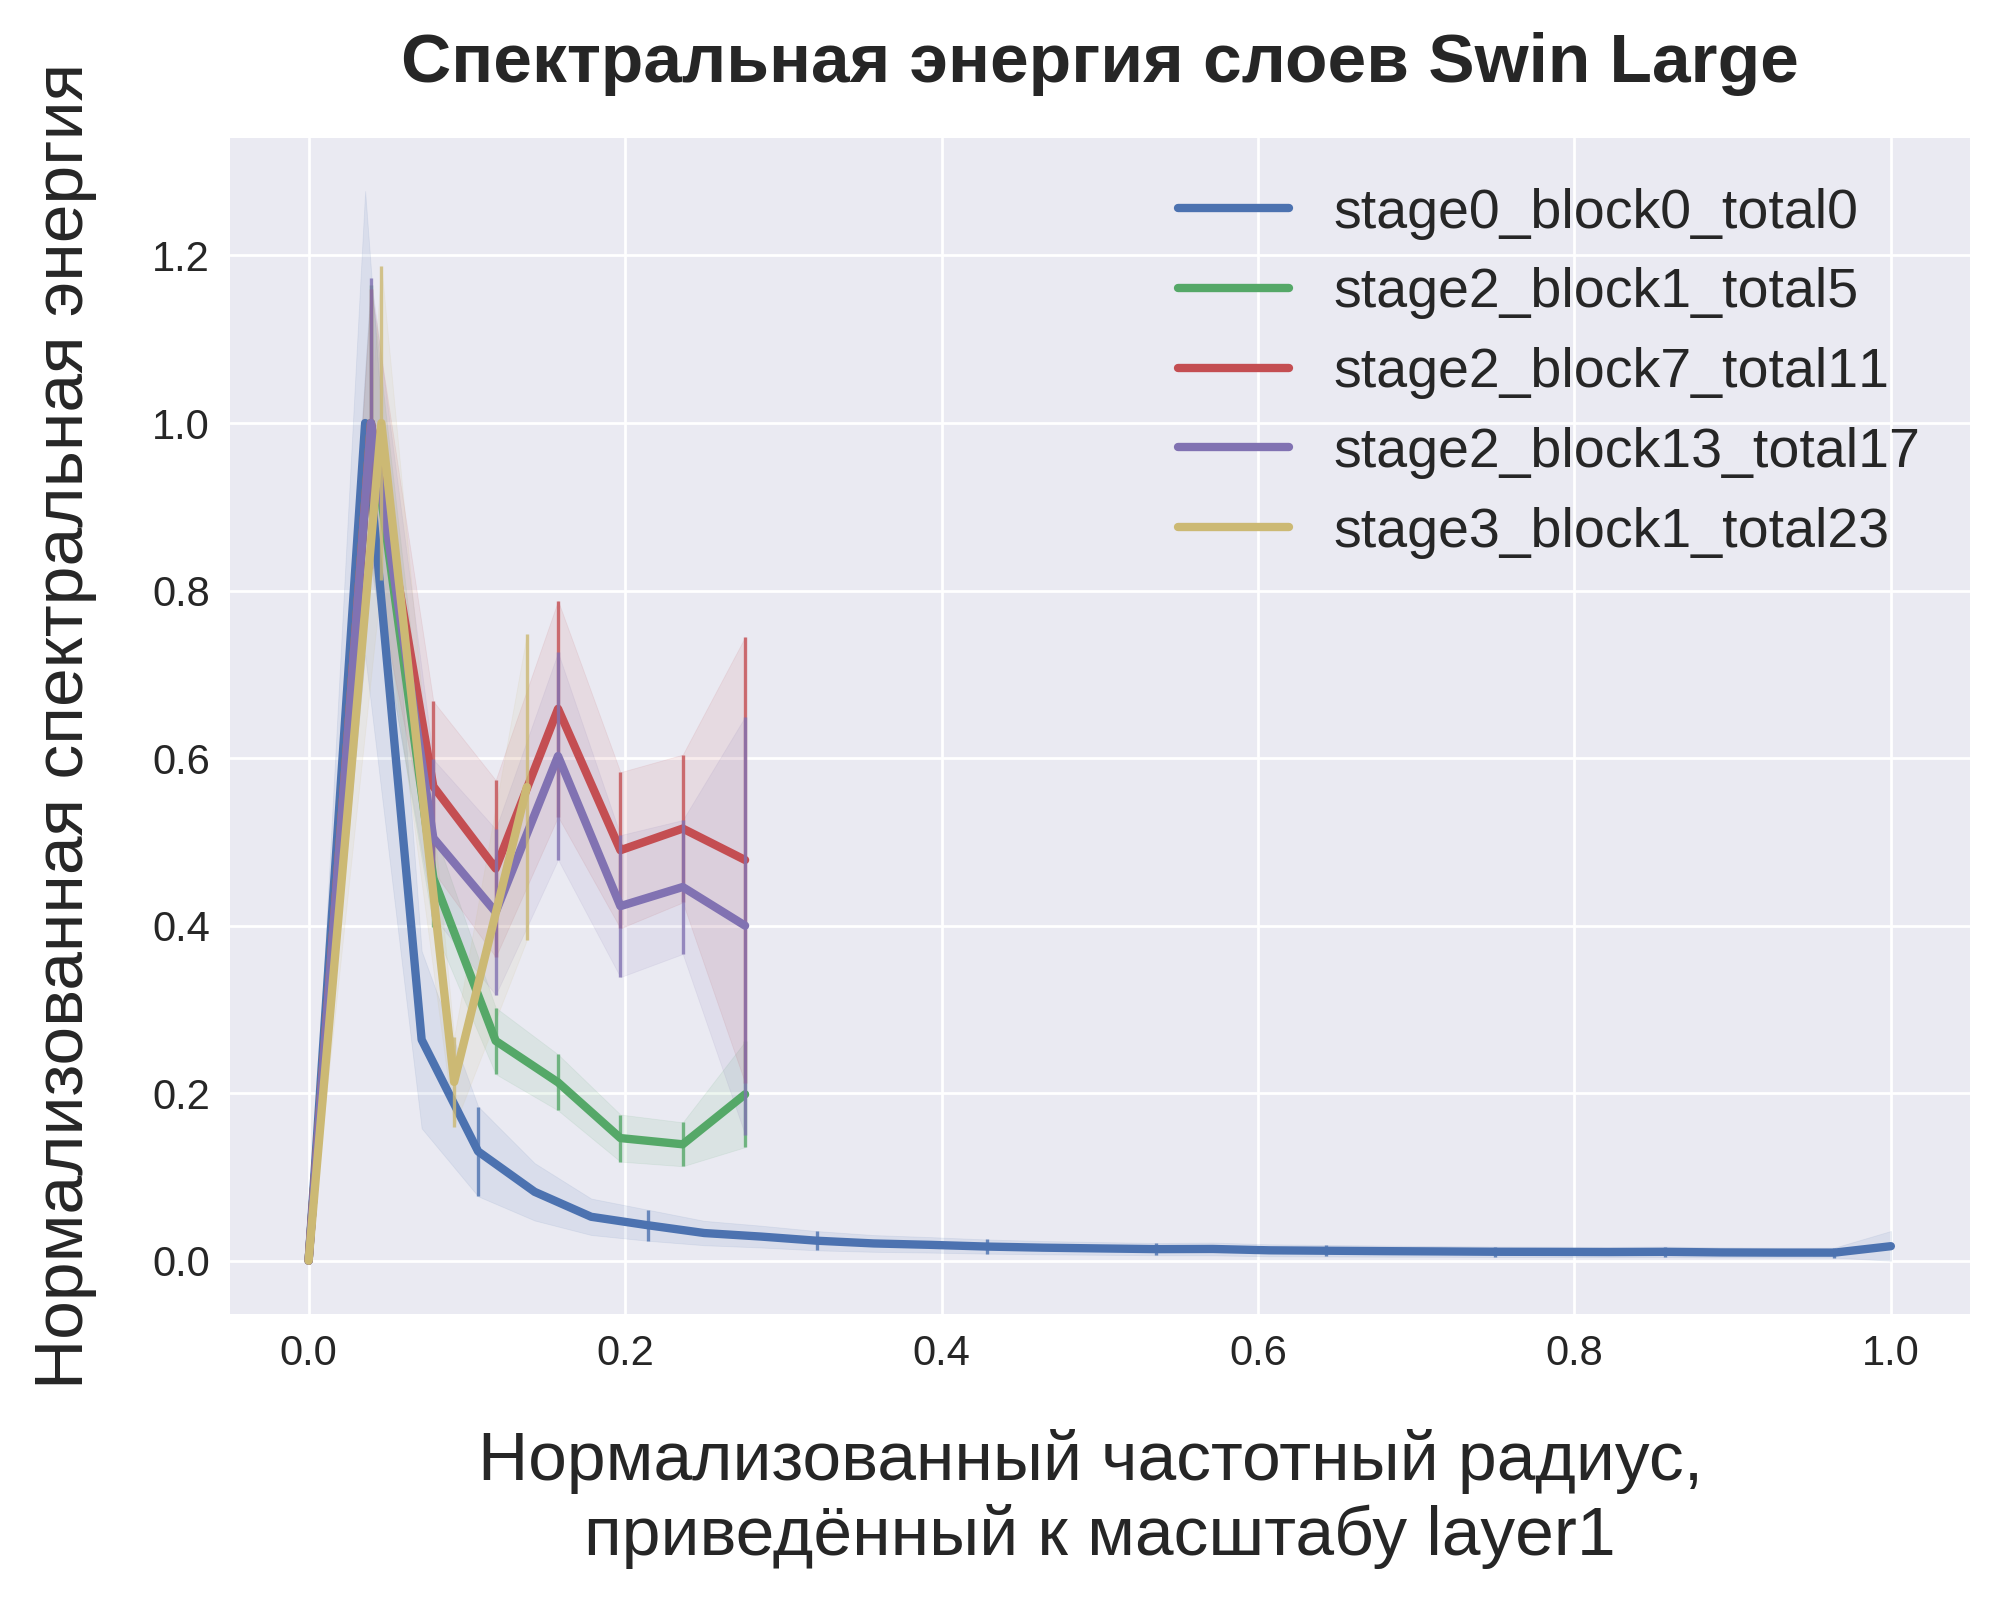
\includegraphics[width=0.8\textwidth]{figures/swin_large_spectra_layers.png}
    \caption{Изменение спектрального профиля по блокам Swin-Large.}
    \label{fig:swin_large_spectra_layers}
\end{figure}

На Рис. \ref{fig:swin_downsampling_control_last_stage} приведён контроль понижения разрешения для Swin-Base. Сравниваются реальный финальный блок и начальное представление, искусственно приведённое к размеру финальной стадии. Этот контроль нужен, потому что в Swin уменьшение разрешения выполняется через \texttt{слияние патчей}, и оно само по себе способно сделать спектр более низкочастотным.

\begin{figure}[h]
    \centering
    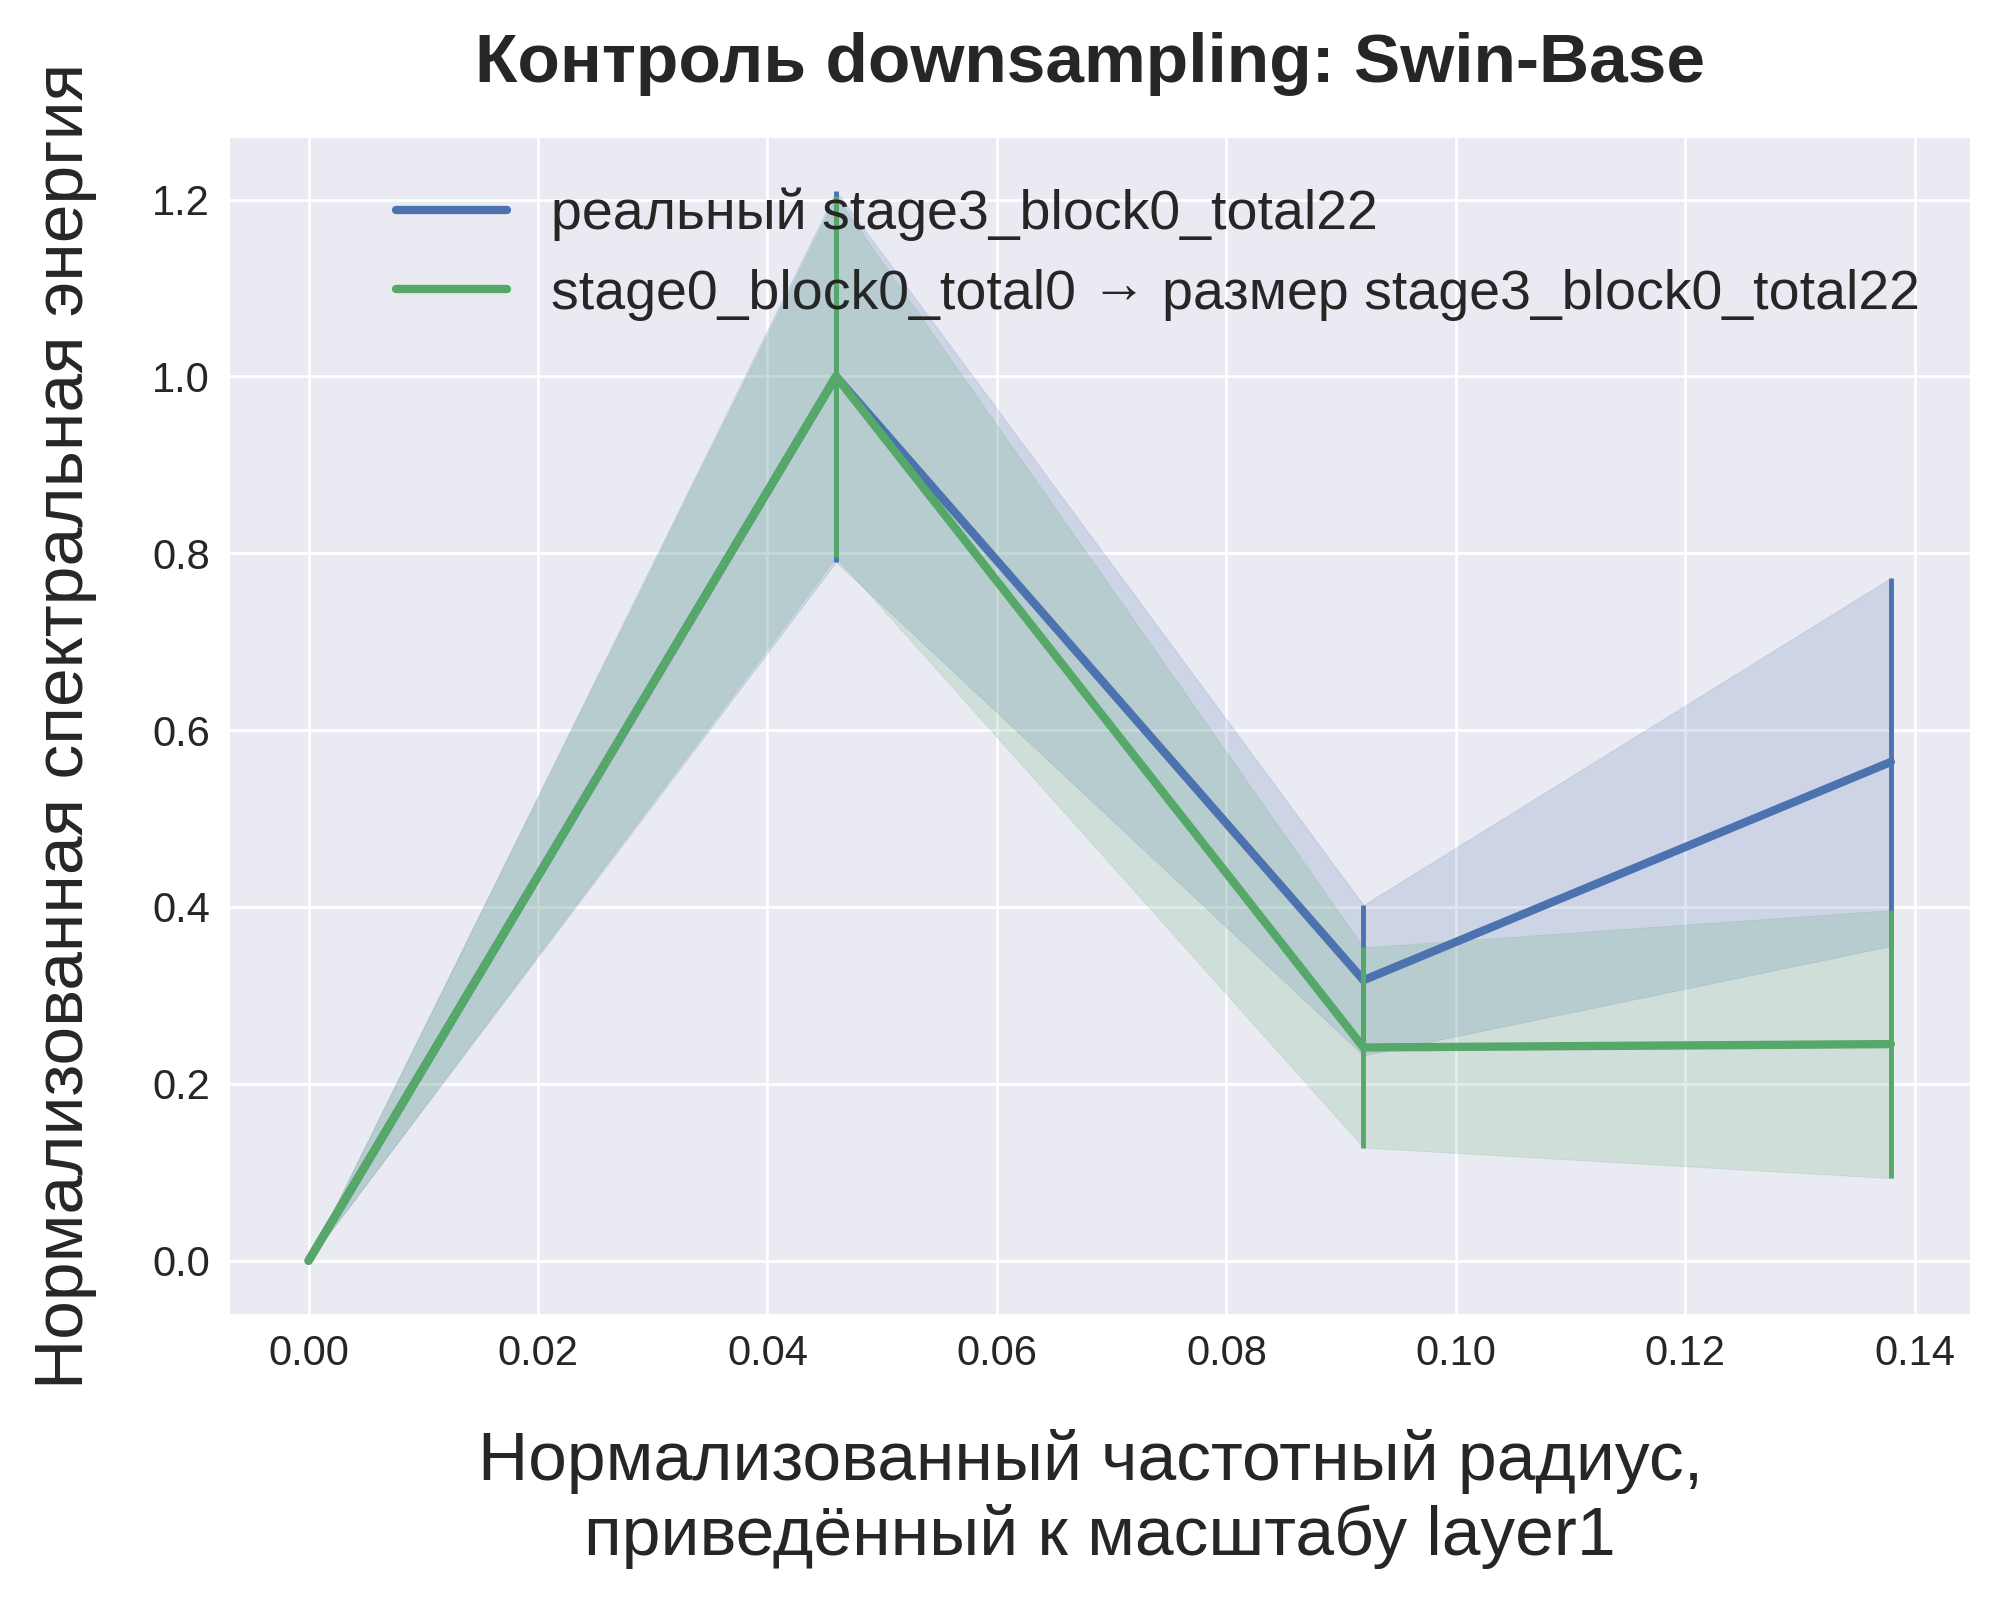
\includegraphics[width=0.8\textwidth]{figures/swin_base_downsampling_control_last_stage.png}
    \caption{Контроль влияния понижения разрешения для Swin-Base: сравнение реального финального блока и начального представления, приведённого к размеру последней стадии.}
    \label{fig:swin_downsampling_control_last_stage}
\end{figure}

Основной пик у двух кривых близок. Значит, уменьшение разрешения действительно объясняет заметную часть финального низкочастотного профиля Swin. Но полного совпадения нет: в хвосте спектра реальная кривая и базовая расходятся. Поэтому вывод по Swin должен быть осторожнее, чем по ResNet. Swin приходит к низкочастотному финальному состоянию, но существенная часть этого эффекта связана с архитектурным уменьшением решётки.



\subsection{Количественная проверка контрольных экспериментов}

Приведённые выше контрольные графики требуют численного уточнения, поскольку визуальное сравнение нормированных кривых показывает только форму спектра. Для этой цели были сопоставлены значения спектрального центроида и доли низкочастотной энергии у реальных представлений и у контрольных представлений, полученных искусственным понижением пространственного разрешения. Такой контроль позволяет проверить, объясняется ли наблюдаемое сужение спектра только уменьшением размера карты признаков.

Для ViT дополнительный контроль пространственного разрешения показывает, что во всех рассмотренных вариантах модели — Tiny, Small, Base и Large — выбранные блоки имеют одинаковую решётку $14 \times 14$, а длина радиального профиля равна $8$. Следовательно, сравнение блоков ViT по глубине не смешивается с изменением пространственного разрешения. Поэтому немонотонная динамика центроида и доли низкочастотной энергии для ViT относится именно к изменению внутренних представлений на фиксированной решётке патчей.

\begin{table}[h]
\centering
\caption{Контроль влияния понижения пространственного разрешения на спектральные метрики}
\label{tab:downsampling_control_metrics}
\vspace{1ex}
\resizebox{\textwidth}{!}{%
\begin{tabular}{llcccccc}
\toprule
\textbf{Модель} & \textbf{Уровень} & \textbf{Центроид} & \textbf{Контроль} & \textbf{$\Delta$} & \textbf{Низкие частоты, \%} & \textbf{Контроль, \%} & \textbf{$\Delta$, п.п.} \\
\midrule
\multirow{3}{*}{ResNet18} 
& \texttt{layer2} & 0.235 $\pm$ 0.014 & 0.251 $\pm$ 0.019 & -0.016 & 34.694 $\pm$ 4.775 & 32.342 $\pm$ 5.919 & +2.352 \\
& \texttt{layer3} & 0.119 $\pm$ 0.006 & 0.132 $\pm$ 0.010 & -0.013 & 64.038 $\pm$ 3.533 & 54.135 $\pm$ 6.241 & +9.903 \\
& \texttt{layer4} & 0.055 $\pm$ 0.002 & 0.074 $\pm$ 0.005 & -0.020 & 100.000 $\pm$ 0.000 & 100.000 $\pm$ 0.000 & 0.000 \\
\midrule
\multirow{3}{*}{Swin-Base}
& \texttt{stage1\_block0} & 0.242 $\pm$ 0.022 & 0.155 $\pm$ 0.037 & +0.086 & 37.006 $\pm$ 6.905 & 64.672 $\pm$ 11.936 & -27.666 \\
& \texttt{stage2\_block0} & 0.130 $\pm$ 0.009 & 0.092 $\pm$ 0.016 & +0.038 & 54.939 $\pm$ 5.443 & 77.424 $\pm$ 8.472 & -22.485 \\
& \texttt{stage3\_block0} & 0.075 $\pm$ 0.007 & 0.067 $\pm$ 0.008 & +0.008 & 100.000 $\pm$ 0.000 & 100.000 $\pm$ 0.000 & 0.000 \\
\bottomrule
\end{tabular}%
}
\end{table}

Таб. \ref{tab:downsampling_control_metrics} показывает, что для ResNet18 реальные представления имеют меньший центроид, чем контрольные представления, полученные простым понижением разрешения. Разность центроида составляет $-0.016$ для \texttt{layer2}, $-0.013$ для \texttt{layer3} и $-0.020$ для \texttt{layer4}. Наиболее показателен \texttt{layer3}: доля низкочастотной энергии в реальном представлении выше контрольного значения на $9.903$ процентного пункта. Это означает, что в ResNet18 сдвиг к низким частотам не сводится к изменению пространственного размера карты признаков.

Для Swin-Base картина отличается. На первых двух стадиях реальные представления имеют больший центроид и меньшую долю низкочастотной энергии, чем контрольные представления. На \texttt{stage1\_block0} разность центроида равна $+0.086$, а доля низкочастотной энергии ниже контрольного значения на $27.666$ процентного пункта. На \texttt{stage2\_block0} соответствующие различия составляют $+0.038$ и $-22.485$ процентного пункта. На третьей стадии разница незначительна и лежит в пределах стандартного отклонения. Следовательно, само понижение разрешения в Swin-Base создаёт более выраженный низкочастотный сдвиг, чем реальные преобразования ранних стадий. Это уточняет интерпретацию Swin: финальный низкочастотный профиль связан с иерархическим уменьшением решётки, но внутренние преобразования модели частично сохраняют средне- и высокочастотные компоненты.

\begin{table}[h]
\centering
\caption{Внутристадийный контроль при фиксированном пространственном разрешении}
\label{tab:within_stage_control_metrics}
\vspace{1ex}
\resizebox{\textwidth}{!}{%
\begin{tabular}{lllccc}
\toprule
\textbf{Модель} & \textbf{Положение} & \textbf{Блок} & \textbf{Центроид} & \textbf{Низкие частоты, \%} & \textbf{Высокие частоты, \%} \\
\midrule
\multirow{3}{*}{ResNet50, \texttt{layer3}} 
& начальный & \texttt{layer3\_block0} & 0.462 $\pm$ 0.024 & 21.431 $\pm$ 4.341 & 43.100 $\pm$ 4.114 \\
& средний & \texttt{layer3\_block3} & 0.438 $\pm$ 0.023 & 23.053 $\pm$ 3.876 & 38.308 $\pm$ 3.918 \\
& глубокий & \texttt{layer3\_block5} & 0.435 $\pm$ 0.021 & 23.117 $\pm$ 3.403 & 37.452 $\pm$ 3.640 \\
\midrule
\multirow{3}{*}{Swin-Base, \texttt{stage2}}
& начальный & \texttt{stage2\_block0} & 0.471 $\pm$ 0.033 & 22.578 $\pm$ 5.910 & 45.061 $\pm$ 5.443 \\
& средний & \texttt{stage2\_block9} & 0.604 $\pm$ 0.014 & 7.497 $\pm$ 1.583 & 69.731 $\pm$ 3.508 \\
& глубокий & \texttt{stage2\_block17} & 0.391 $\pm$ 0.051 & 26.830 $\pm$ 6.676 & 28.748 $\pm$ 9.955 \\
\bottomrule
\end{tabular}%
}
\end{table}

Таб. \ref{tab:within_stage_control_metrics} дополняет предыдущий контроль, поскольку в ней сравниваются блоки внутри одной стадии, то есть при фиксированном пространственном разрешении. Для ResNet50 внутри \texttt{layer3} наблюдается умеренное снижение центроида с $0.462 \pm 0.024$ до $0.435 \pm 0.021$ и уменьшение доли высокочастотной энергии с $43.100 \pm 4.114\%$ до $37.452 \pm 3.640\%$. Эти изменения слабее межстадийных различий, но они показывают, что спектральное сжатие в ResNet присутствует и внутри стадии.

Для Swin-Base внутри \texttt{stage2} динамика оказывается немонотонной. Средний блок имеет больший центроид, чем начальный: $0.604 \pm 0.014$ против $0.471 \pm 0.033$, а доля высокочастотной энергии возрастает с $45.061 \pm 5.443\%$ до $69.731 \pm 3.508\%$. В глубоком блоке центроид снижается до $0.391 \pm 0.051$, а доля высокочастотной энергии уменьшается до $28.748 \pm 9.955\%$. Следовательно, внутри одной стадии Swin-Base не демонстрирует простого последовательного сжатия спектра: сначала происходит усиление более высокочастотной составляющей, а затем выраженный сдвиг к низким частотам.

В совокупности контрольные эксперименты показывают, что наблюдаемая спектральная динамика не является только следствием изменения пространственного разрешения. Для ResNet низкочастотный сдвиг усиливается внутренними преобразованиями сети, для ViT сравнение выполняется на фиксированной решётке патчей, а для Swin влияние понижения разрешения и внутренних преобразований имеет различный характер на разных стадиях.

\subsection{Межсемейственное сравнение архитектур}

На Рис. \ref{fig:compare_begin_block} показаны нормализованные радиальные спектры мощности для начальных уровней ResNet, ViT и Swin. У всех семейств максимум находится в области малых частотных радиусов. Значит, уже в начале обработки основная энергия признаков сосредоточена около низких частот.

При этом кривые не совпадают. У ResNet хвост после основного пика выглядит более протяжённым: начальные свёрточные признаки ещё несут часть локальной текстурной информации. У ViT и Swin начальные представления формируются не как плотные пиксельные карты признаков, а через патчи и токены. Поэтому их спектральный профиль задаётся другой пространственной дискретизацией. На этом уровне различия между архитектурами ещё не максимальны, но видно, что каждая из них стартует с собственной формой распределения энергии.

\begin{figure}[h]
    \centering
    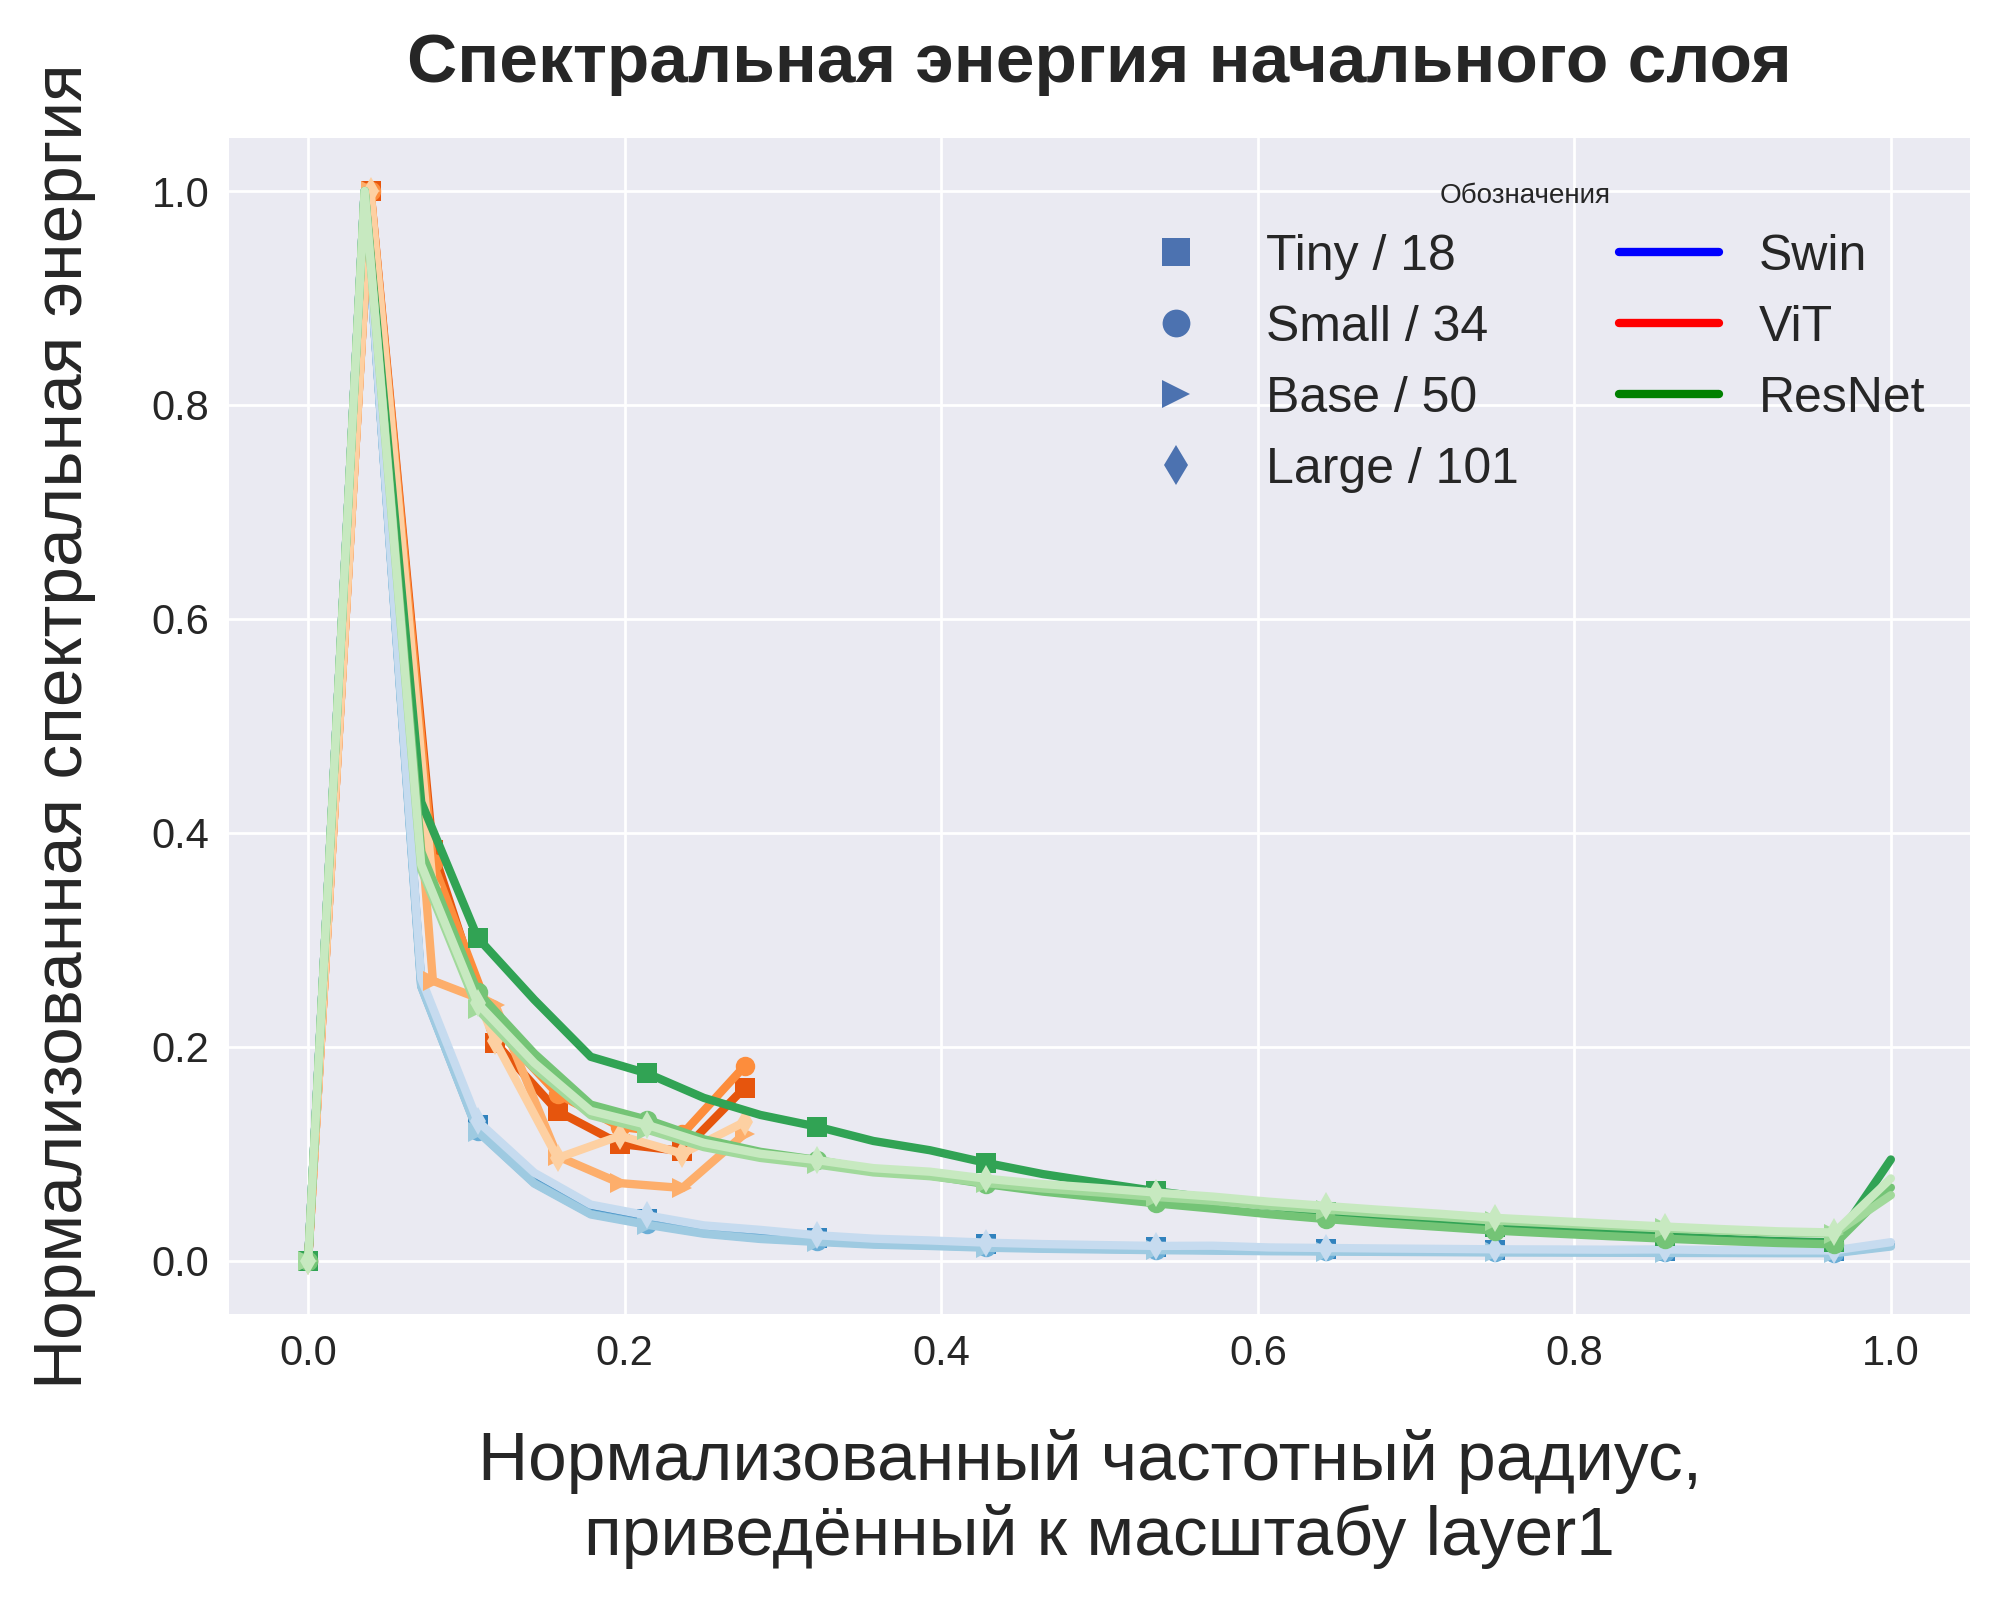
\includegraphics[width=0.8\textwidth]{figures/compare_begin_block.png}
    \caption{Сравнение радиальных спектров мощности начальных уровней ResNet, ViT и Swin.}
    \label{fig:compare_begin_block}
\end{figure}

На средних уровнях различия становятся заметнее (Рис. \ref{fig:compare_middle_block}). ResNet быстрее смещается к низкочастотной области: после пика энергия падает достаточно резко. ViT и Swin ведут себя менее однородно. У части кривых сохраняется более высокий хвост в среднечастотной области, а у некоторых моделей видны локальные подъёмы в правой части рассматриваемого диапазона.

Этот график полезен тем, что показывает не только «кто шире», но и насколько по-разному устроена середина моделей. ResNet к этому моменту уже в значительной степени агрегирует признаки. ViT сохраняет более свободную динамику на фиксированной решётке патчей. Swin находится между ними: он иерархичен, но на средних стадиях не выглядит полностью свёрточным.

\begin{figure}[h]
    \centering
    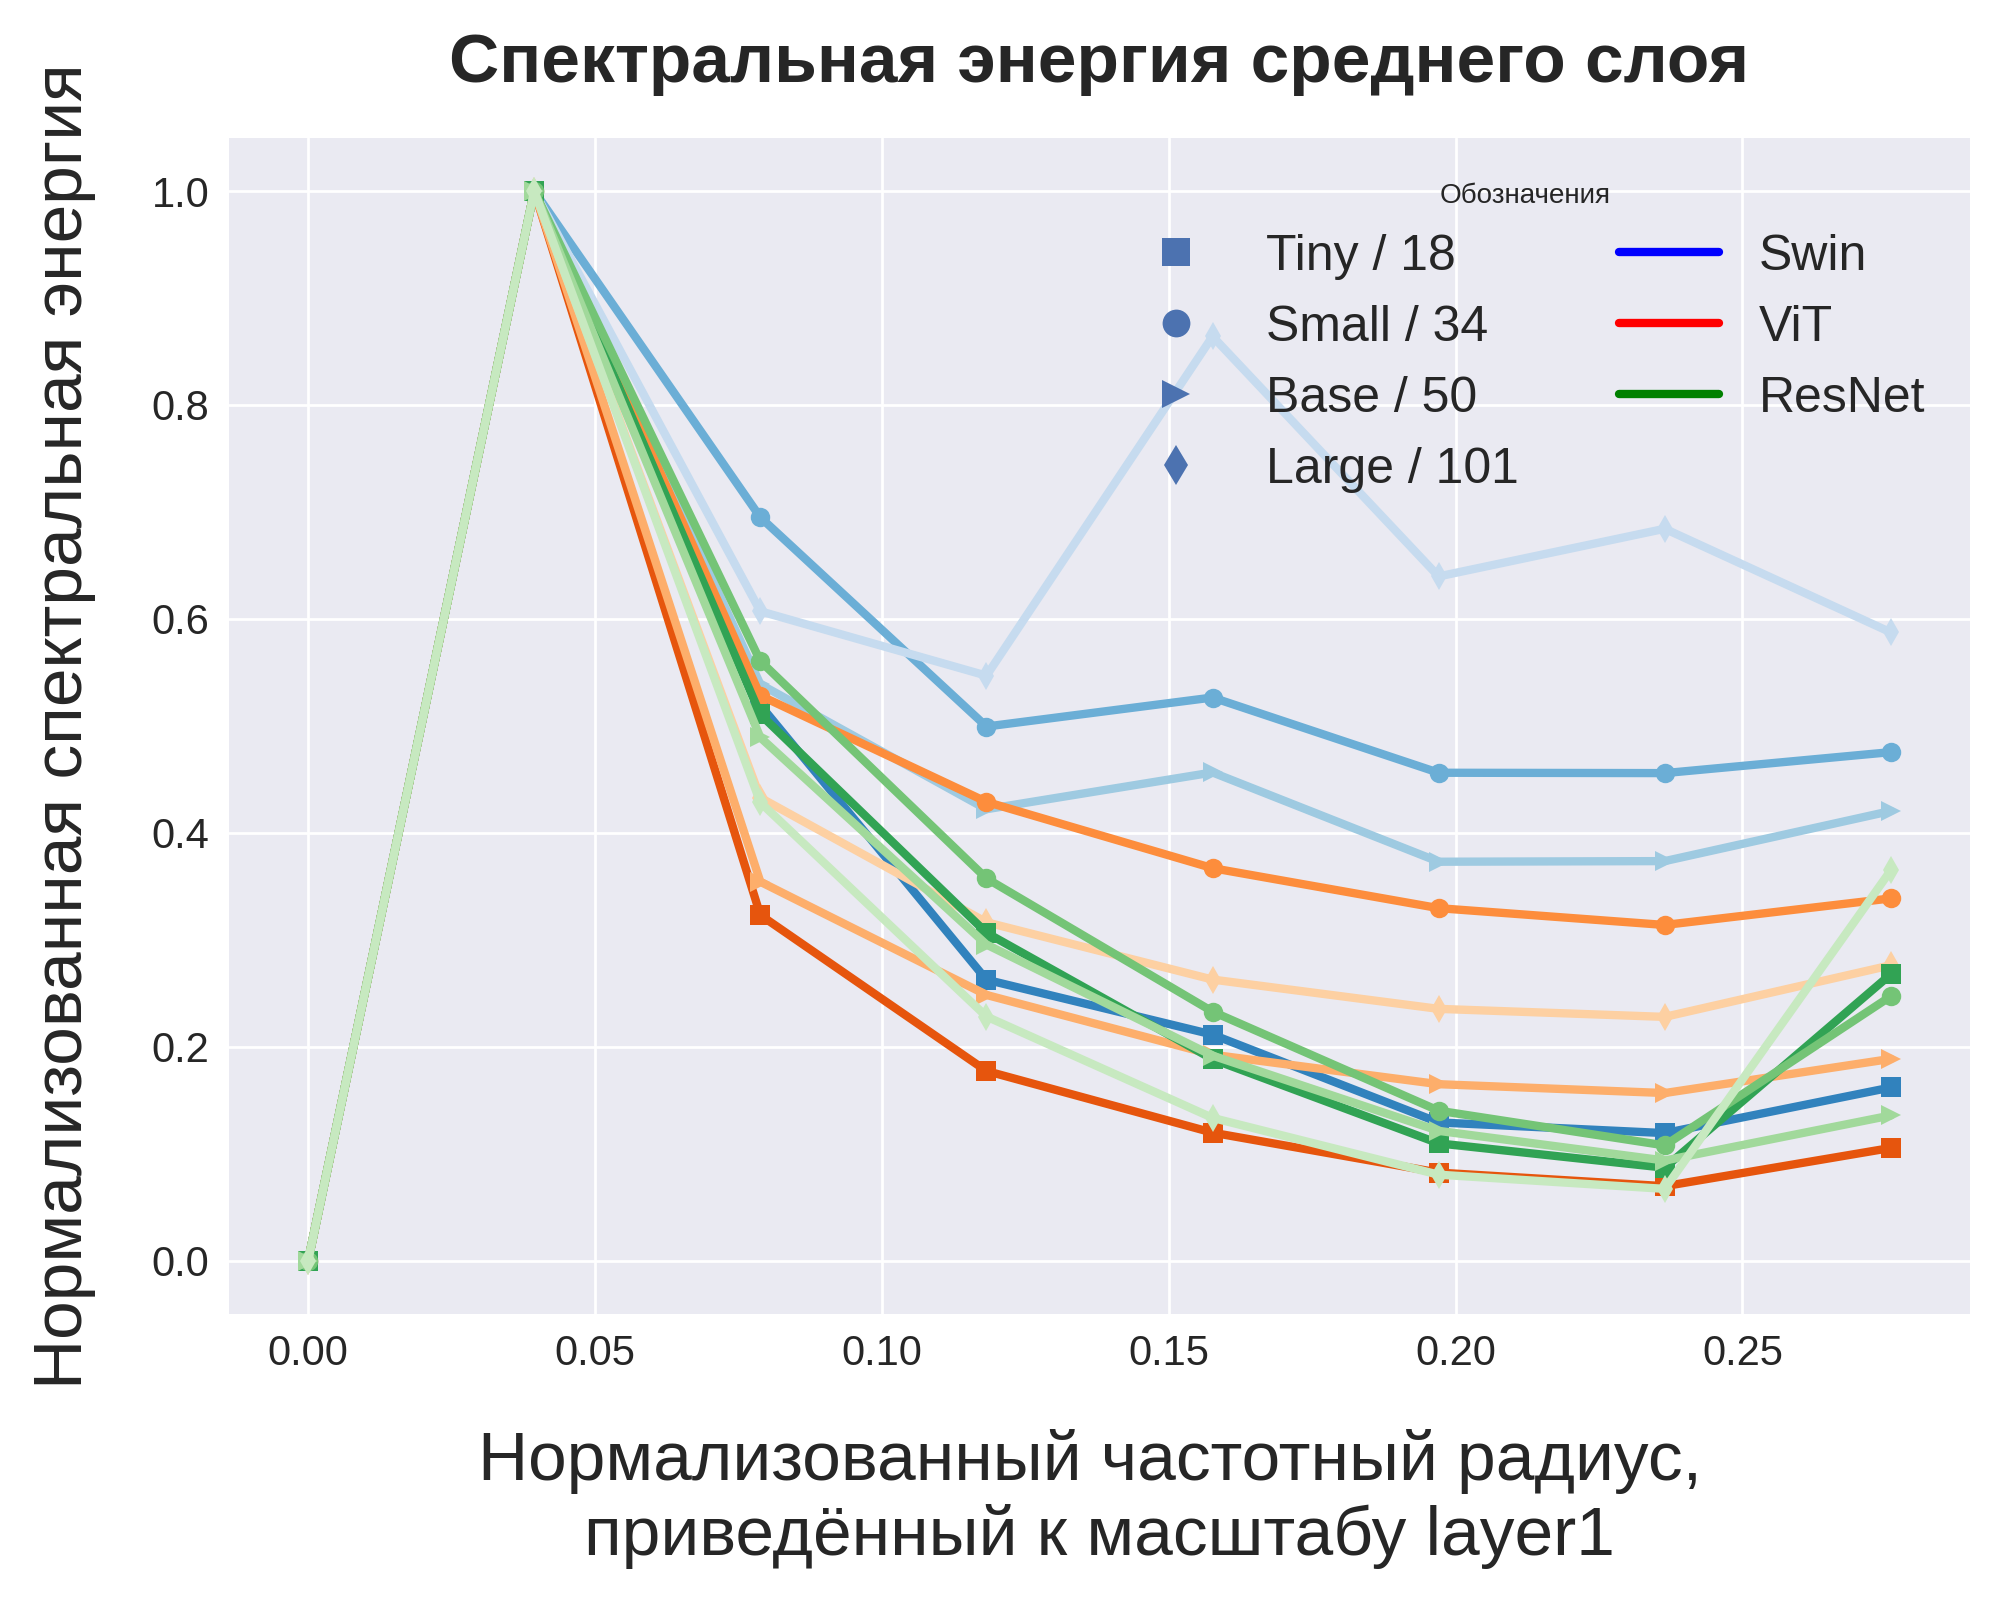
\includegraphics[width=0.8\textwidth]{figures/compare_middle_block.png}
    \caption{Сравнение радиальных спектров мощности средних уровней ResNet, ViT и Swin.}
    \label{fig:compare_middle_block}
\end{figure}

На Рис. \ref{fig:compare_last_block} сравниваются последние уровни моделей. ResNet имеет наиболее узкий финальный профиль: после основного пика энергия быстро падает, а хвост остаётся небольшим. ViT показывает более неоднородную картину. У части моделей финальный спектр остаётся достаточно широким, особенно у крупных вариантов. Swin, по форме, занимает промежуточное положение: финальные кривые уже ограничены по частотному диапазону, но не совпадают полностью с ResNet.

На графиках у некоторых кривых виден небольшой подъём хвоста у правой границы. Это не нужно интерпретировать как содержательное усиление самых высоких частот. Такой эффект связан с обработкой частотной плоскости внутри круга Найквиста и с тем, что в крайних радиальных кольцах остаётся меньше точек, а нормировка кривых по максимуму делает малые колебания более заметными. На численные выводы это влияет слабо: метрики рассчитываются по суммарной энергии кольца, а не только по визуальной форме нормированной кривой. Поэтому правый край графика в этой работе используется осторожно; основной смысл несут положение центроида, доля энергии в низких частотах и общая форма спада после пика.

\begin{figure}[h!]
    \centering
    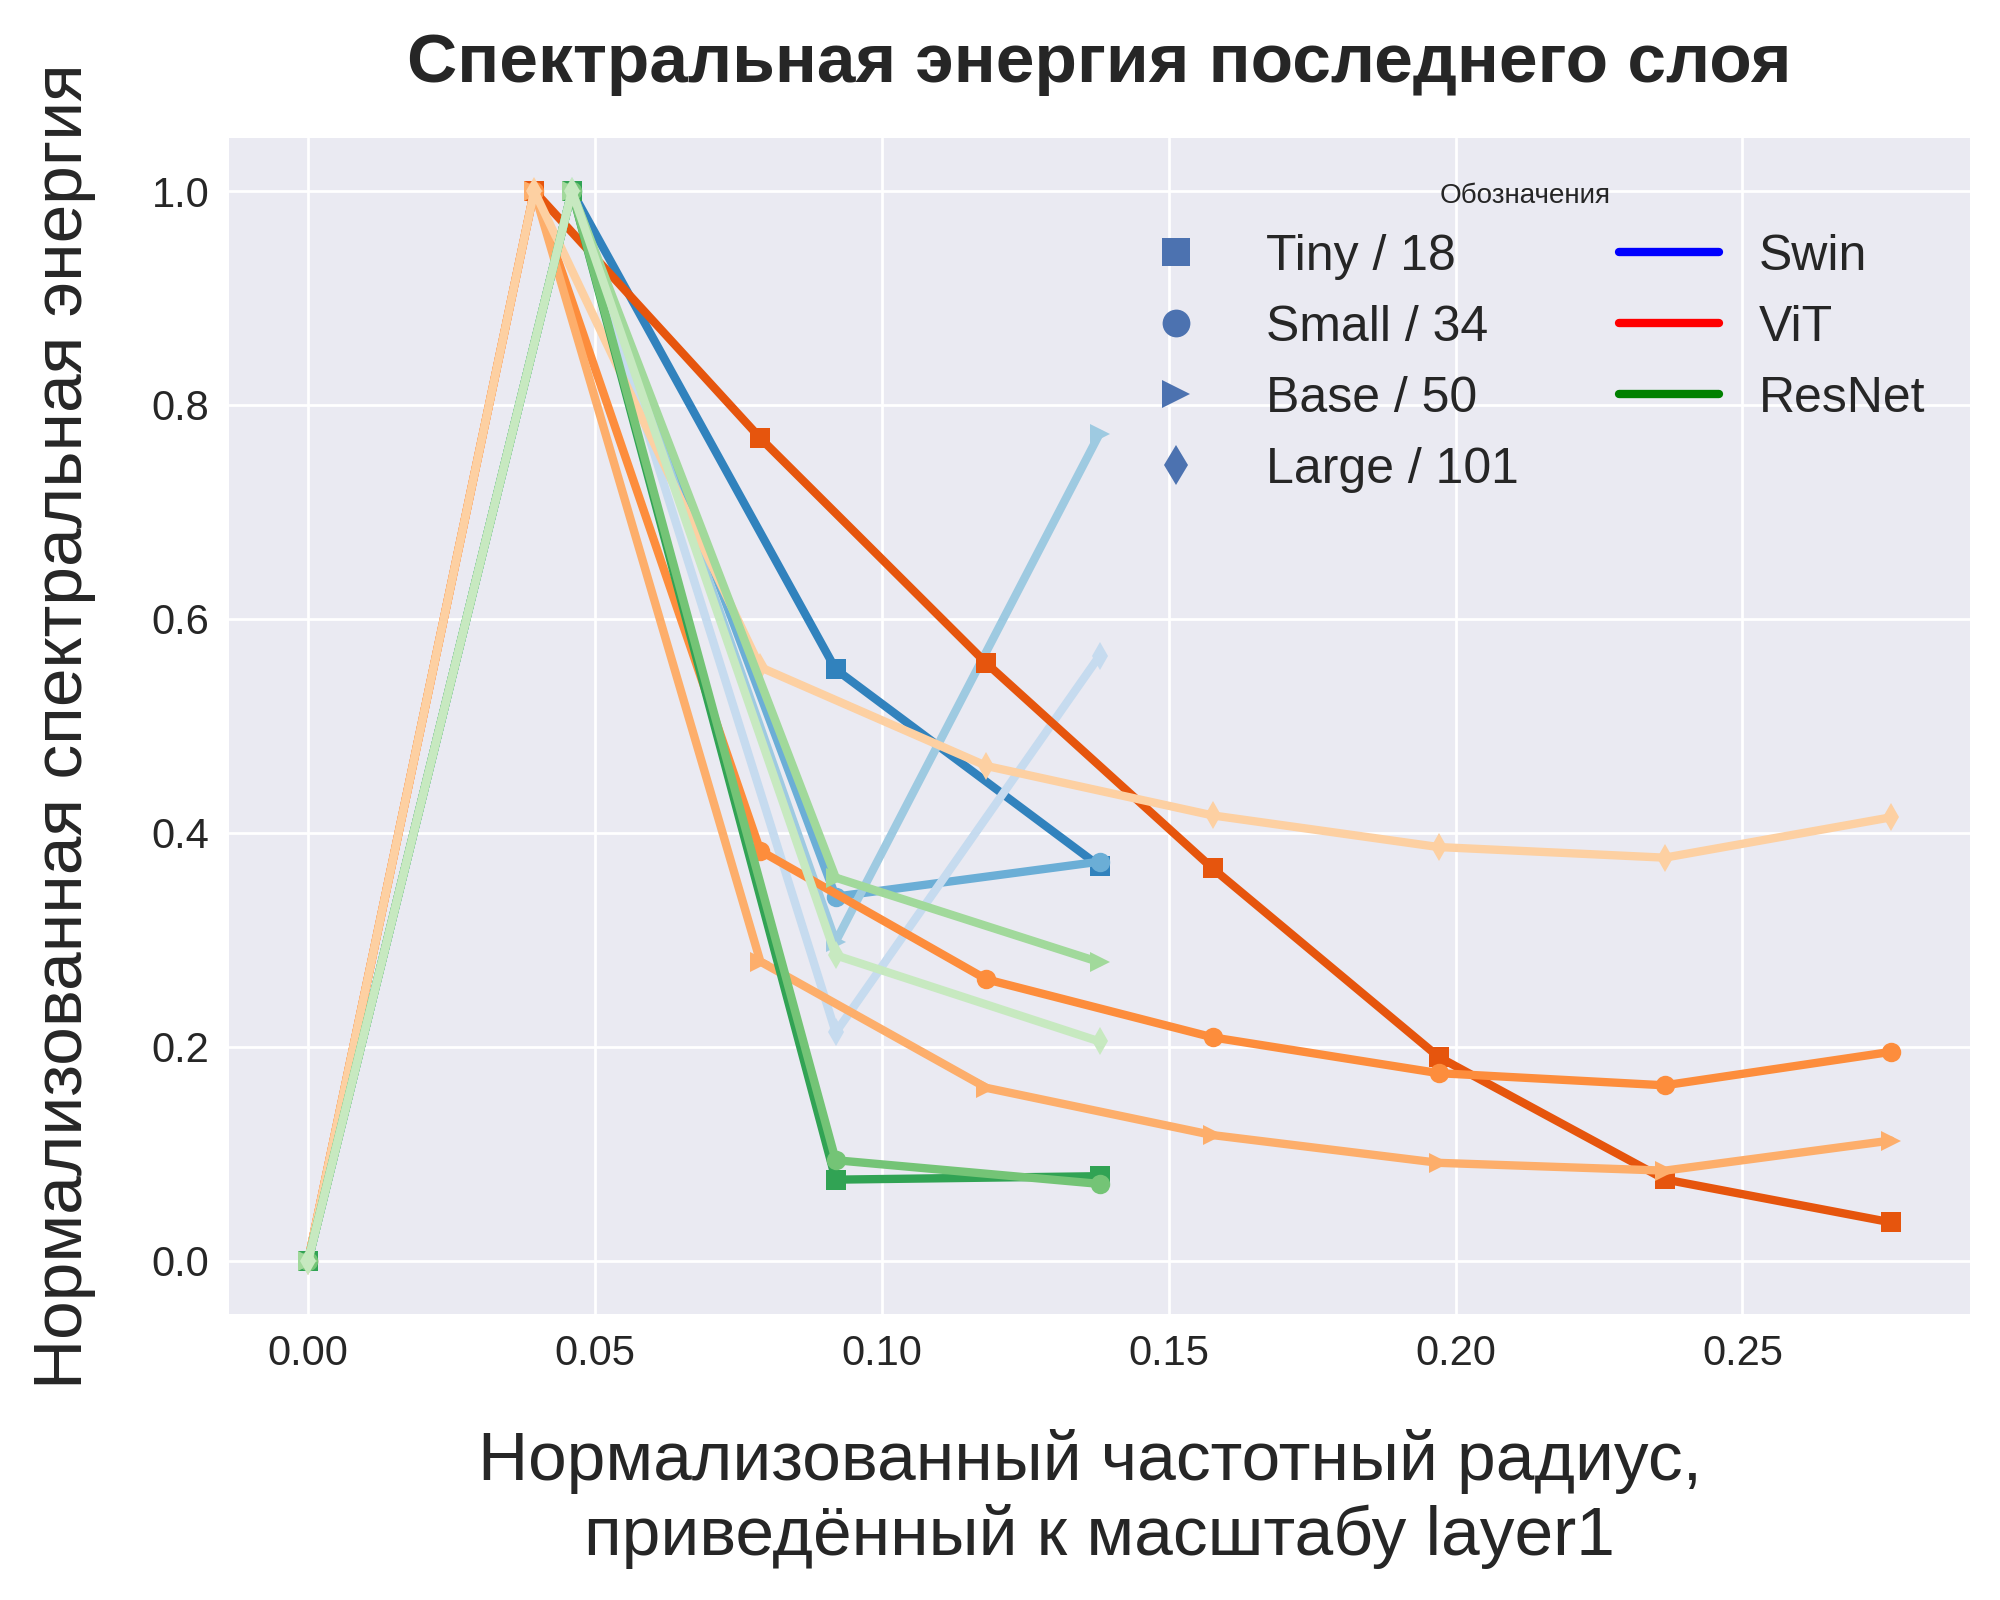
\includegraphics[width=0.8\textwidth]{figures/compare_last_block.png}
    \caption{Сравнение радиальных спектров мощности последних уровней ResNet, ViT и Swin.}
    \label{fig:compare_last_block}
\end{figure}

По графикам видно, что трансформерные архитектуры не повторяют спектральную динамику CNN. ResNet даёт наиболее последовательное сжатие спектра, ViT показывает более свободное перераспределение энергии, а Swin оказывается между ними. Но после контрольных экспериментов этот вывод звучит точнее: для ResNet и Swin часть сужения связана с уменьшением пространственного разрешения, тогда как для ViT такая причина между блоками отсутствует.

\section{Сводная интерпретация по метрикам}

Для численного сравнения использовались три показателя: спектральный центроид, доля низкочастотной энергии и скорость спектрального сжатия. Графики дают форму кривой, а метрики позволяют проверить те же наблюдения в компактном виде. Значения в таблицах приведены в формате среднее $\pm$ стандартное отклонение по изображениям выборки.

В Таб. \ref{tab:SpectraCentr_metrics} приведены значения спектрального центроида для моделей разных семейств. У ResNet картина самая ровная: центроид уменьшается от начальных уровней к глубоким во всех четырёх моделях. Для ResNet18 он снижается с $0.431\pm0.034$ до $0.055\pm0.002$, для ResNet34 — с $0.436\pm0.036$ до $0.056\pm0.002$, для ResNet50 — с $0.480\pm0.034$ до $0.071\pm0.004$, для ResNet101 — с $0.484\pm0.032$ до $0.067\pm0.004$. Это численно подтверждает то, что было видно на графиках: по глубине ResNet сдвигает энергию к меньшим частотным радиусам.

Есть и небольшая деталь. У ResNet50 и ResNet101 начальный центроид выше, чем у ResNet18/34. Возможно, это связано с более широкой и сложной структурой bottleneck-блоков. Но к финальным уровням все модели приходят к близкому диапазону. Значит, более глубокая ResNet меняет траекторию сжатия, но итоговый низкочастотный характер остаётся общим для всего семейства.

\begin{table}[h]
\centering
\caption{Спектральный центроид различных архитектур} 
\label{tab:SpectraCentr_metrics}
\vspace{1ex} 
\begin{tabular}{llccc}
\toprule
\textbf{Архитектура} & \textbf{Тип} & \textbf{Начальные} & \textbf{Средние} & \textbf{Глубокие} \\
\midrule

\multirow{4}{*}{CNN} & resnet18      & 0.431 $\pm$ 0.034 & 0.119 $\pm$ 0.006 & 0.055 $\pm$ 0.002 \\
                     & resnet34      & 0.436 $\pm$ 0.036 & 0.123 $\pm$ 0.006 & 0.056 $\pm$ 0.002 \\
                     & resnet50      & 0.480 $\pm$ 0.034 & 0.120 $\pm$ 0.006 & 0.071 $\pm$ 0.004 \\
                     & resnet101     & 0.484 $\pm$ 0.032 & 0.114 $\pm$ 0.005 & 0.067 $\pm$ 0.004 \\

\midrule

\multirow{4}{*}{ViT} & Tiny      & 0.120 $\pm$ 0.011 & 0.112 $\pm$ 0.010 & 0.121 $\pm$ 0.004 \\
                     & Small     & 0.125 $\pm$ 0.011 & 0.149 $\pm$ 0.013 & 0.134 $\pm$ 0.011 \\
                     & Base      & 0.112 $\pm$ 0.008 & 0.133 $\pm$ 0.012 & 0.117 $\pm$ 0.013 \\
                     & Large     & 0.121 $\pm$ 0.007 & 0.143 $\pm$ 0.007 & 0.154 $\pm$ 0.007 \\
\midrule

\multirow{4}{*}{Swin} & Tiny       & 0.369 $\pm$ 0.086 & 0.124 $\pm$ 0.007 & 0.075 $\pm$ 0.006 \\
                      & Small      & 0.348 $\pm$ 0.091 & 0.156 $\pm$ 0.005 & 0.072 $\pm$ 0.007 \\
                      & Base       & 0.340 $\pm$ 0.090 & 0.154 $\pm$ 0.004 & 0.078 $\pm$ 0.010 \\
                      & Large      & 0.383 $\pm$ 0.079 & 0.167 $\pm$ 0.004 & 0.073 $\pm$ 0.007 \\
\bottomrule
\end{tabular}
\end{table}

У ViT значения центроида лежат в более узком диапазоне, но ведут себя менее регулярно по глубине. У Tiny центроид практически возвращается к начальному уровню: $0.120\pm0.011$ в начале и $0.121\pm0.004$ на глубоком блоке. У Small и Base максимум приходится на средний уровень. У Large центроид растёт от $0.121\pm0.007$ до $0.154\pm0.007$. Такая динамика не похожа на устойчивое подавление средних частот. Скорее ViT перераспределяет энергию между блоками, а не просто сжимает её к низкочастотной области.

У Swin центроид заметно снижается к глубоким блокам: финальные значения лежат в диапазоне $0.072$--$0.078$. При этом средний уровень у Swin ведёт себя не полностью одинаково для всех масштабов: у Tiny центроид ниже, чем у Small/Base/Large. Это согласуется с графиками: Swin действительно приходит к низкочастотному финальному состоянию, но промежуточная динамика у него сложнее, чем у ResNet, и сильнее зависит от стадии.

В Таб. \ref{tab:LowFrac_metrics} приведена доля низкочастотной энергии при пороге $\rho<0.15$. Для CNN эта метрика растёт во всех моделях. У ResNet18 значение увеличивается с $17.832\pm4.562$ до $100.000\pm0.000$, у ResNet34 — с $19.230\pm4.878$ до $100.000\pm0.000$, у ResNet50 — с $16.692\pm4.354$ до $100.000\pm0.000$, у ResNet101 — с $16.051\pm4.066$ до $100.000\pm0.000$. Здесь центроид и доля низких частот дают согласованную картину: спектр ResNet по глубине сжимается, а низкочастотная область получает всё больший вес.

При этом значение $100\%$ на глубоких уровнях не надо понимать как «вся информация стала низкочастотной» в содержательном смысле. Оно возникает потому, что после приведения частотной оси к масштабу \texttt{layer1} доступный диапазон глубоких карт ResNet полностью попадает ниже выбранного порога $\rho<0.15$. Поэтому эта метрика здесь одновременно отражает и спектральную концентрацию, и эффект уменьшения пространственного разрешения. Именно поэтому выше был добавлен контроль понижения разрешения.

\begin{table}[h]
\centering
\caption{Доля низкочастотной энергии различных архитектур, \%} 
\label{tab:LowFrac_metrics}
\vspace{1ex} 
\begin{tabular}{llccc}
\toprule
\textbf{Архитектура} & \textbf{Тип} & \textbf{Начальные} & \textbf{Средние} & \textbf{Глубокие} \\
\midrule

\multirow{4}{*}{CNN} & resnet18      & 17.832 $\pm$ 4.562 & 64.038 $\pm$ 3.533 & 100.000 $\pm$ 0.000 \\
                     & resnet34      & 19.230 $\pm$ 4.878 & 60.876 $\pm$ 3.543 & 100.000 $\pm$ 0.000 \\
                     & resnet50      & 16.692 $\pm$ 4.354 & 62.548 $\pm$ 3.640 & 100.000 $\pm$ 0.000 \\
                     & resnet101     & 16.051 $\pm$ 4.066 & 67.072 $\pm$ 3.017 & 100.000 $\pm$ 0.000 \\

\midrule

\multirow{4}{*}{ViT} & Tiny      & 61.314 $\pm$ 6.542 & 65.695 $\pm$ 5.778 & 62.119 $\pm$ 3.112 \\
                     & Small     & 58.272 $\pm$ 6.399 & 43.058 $\pm$ 8.355 & 51.924 $\pm$ 6.795 \\
                     & Base      & 68.402 $\pm$ 4.884 & 52.567 $\pm$ 7.525 & 62.402 $\pm$ 7.364 \\
                     & Large     & 62.201 $\pm$ 4.225 & 46.683 $\pm$ 4.687 & 39.819 $\pm$ 4.989 \\
\midrule

\multirow{4}{*}{Swin} & Tiny       & 39.189 $\pm$ 13.636 & 59.380 $\pm$ 4.247 & 100.000 $\pm$ 0.000 \\
                      & Small      & 43.009 $\pm$ 14.656 & 37.743 $\pm$ 3.771 & 100.000 $\pm$ 0.000 \\
                      & Base       & 44.194 $\pm$ 14.614 & 38.511 $\pm$ 3.146 & 100.000 $\pm$ 0.000 \\
                      & Large      & 36.661 $\pm$ 12.507 & 28.543 $\pm$ 3.607 & 100.000 $\pm$ 0.000 \\
\bottomrule
\end{tabular}
\end{table}

У ViT единой траектории нет. У Tiny доля низкочастотной энергии остаётся примерно на одном уровне: $61.314\pm6.542$ в начале и $62.119\pm3.112$ на глубоком блоке. У Small и Base видно снижение на среднем уровне и частичное восстановление к глубокому. У Large доля низких частот падает почти последовательно — с $62.201\pm4.225$ до $39.819\pm4.989$. Это ещё раз показывает: ViT нельзя описать одной простой схемой низкочастотного накопления.

У Swin доля низких частот к глубоким блокам также доходит до $100\%$ при выбранном пороге. Здесь причина похожа на ResNet: финальная стадия имеет меньшую решётку, и после приведения к масштабу начального уровня доступные радиусы оказываются внутри низкочастотного диапазона. Поэтому вывод по Swin нельзя делать только по этой таблице. Нужно совместно учитывать центроид, форму кривых и контроль понижения разрешения.

Таб. \ref{tab:models_metrics} показывает скорость спектрального сжатия в экспоненциальной модели (Уравнение \ref{eq:slope})  У CNN значения $\lambda$ наиболее высокие: от $1.930$ до $2.028$. Это согласуется с графиками и таблицей центроидов: ResNet демонстрирует наиболее выраженное снижение спектрального центроида по глубине. При этом разброс значений относительно небольшой, то есть такой режим характерен для всех рассмотренных моделей семейства.

У ViT коэффициент близок к нулю или отрицателен. Для Tiny он равен $-0.103 \pm 0.132$, то есть почти не отличается от нуля с учётом погрешности. Для Large значение составляет $-0.334 \pm 0.078$, что уже указывает на рост центроида по глубине. Поэтому ViT нельзя описывать как архитектуру с экспоненциальным низкочастотным сжатием: в данном эксперименте его спектральная динамика остаётся немонотонной.

У Swin значения $\lambda$ положительные и лежат в диапазоне от $0.951$ до $1.774$. По этой метрике Swin оказывается ближе к ResNet, чем к ViT: центроид у него в среднем снижается по глубине. Однако этот результат нужно читать вместе с контрольным экспериментом, поскольку часть снижения у Swin связана с уменьшением пространственной решётки через \texttt{слияние патчей}.

\begin{table}[h]
\centering
\caption{Коэффициент экспоненциального спектрального сжатия $\lambda$}
\label{tab:models_metrics}
\vspace{1ex}

\begin{tabular}{ccccc}
\toprule
\textbf{Архитектура} & \textbf{Tiny(18)} & \textbf{Small(34)} & \textbf{Base(50)} & \textbf{Large(101)} \\
\midrule
CNN & 1.930 $\pm$ 0.109 & 1.954 $\pm$ 0.115 & 2.019 $\pm$ 0.098 & 2.028 $\pm$ 0.085 \\
ViT & -0.103 $\pm$ 0.132 & -0.206 $\pm$ 0.115 & -0.078 $\pm$ 0.112 & -0.334 $\pm$ 0.078 \\
Swin & 1.774 $\pm$ 0.426 & 1.063 $\pm$ 0.365 & 0.951 $\pm$ 0.353 & 1.171 $\pm$ 0.312 \\
\bottomrule
\end{tabular}
\end{table}

Сопоставление трёх таблиц даёт общий вывод по метрикам. ResNet демонстрирует наиболее устойчивое снижение центроида и рост низкочастотной доли. ViT показывает немонотонную динамику: коэффициент $\lambda$ у него близок к нулю или отрицателен, поэтому модель нельзя описать как архитектуру с последовательным экспоненциальным сжатием спектра. Swin по значениям $\lambda$ занимает промежуточное положение: снижение центроида выражено достаточно заметно, но контроль понижения разрешения показывает, что для него особенно важен вклад уменьшения пространственного разрешения.

\section{Обобщение экспериментальных результатов}

Совместный анализ графиков и таблиц показывает, что архитектуры различаются не только числом параметров. Они по-разному меняют частотный состав внутренних представлений. Это видно уже на уровне спектральных кривых, а затем подтверждается центроидом, долей низких частот и скоростью сжатия.

Для ResNet наблюдается самый понятный сценарий. Центроид падает, доля низкочастотной энергии растёт, скорость сжатия положительна во всех вариантах. Однако теперь этот вывод нужно формулировать точнее: часть низкочастотного сдвига связана с уменьшением пространственного разрешения между стадиями. Контрольный эксперимент показывает, что понижение разрешения не объясняет всё полностью, потому что реальный \texttt{layer4} заметно уже, чем искусственно уменьшенный \texttt{layer1}. Поэтому для ResNet корректнее говорить о совместном эффекте архитектурной иерархии и изменения самих признаков.

ViT ведёт себя иначе. Его центроид может расти на средних или поздних блоках, а доля низких частот меняется без единого шаблона. Это не является локальным исключением: изображение обрабатывается как последовательность патчей, и блоки модели не обязаны давать монотонное спектральное сжатие. При этом в работе не утверждается, что причина связана только с механизмом внимания. По данным эксперимента можно сказать более строго: при фиксированной патчевой решётке ViT перераспределяет спектральную энергию немонотонно.

Swin занимает промежуточное место. На глубоких блоках он приходит к низким значениям центроида и высокой доле низкочастотной энергии, то есть финально сближается с CNN. Но контроль понижения разрешения показывает, что значительная часть этого сближения связана с уменьшением решётки через \texttt{слияние патчей}. При этом графики средних стадий говорят, что Swin всё же не является простой копией ResNet: внутри сети есть участки с более широким спектральным профилем.

Главный экспериментальный результат можно сформулировать так: ResNet даёт наиболее последовательное низкочастотное сжатие, ViT — немонотонное перераспределение спектральной энергии при фиксированной решётке патчей, Swin — финальный низкочастотный профиль, который частично объясняется понижением разрешения. Архитектура задаёт не только конечную форму представления, но и сам путь перераспределения энергии по глубине.
